\documentclass[12pt,letterpaper]{article}
%\usepackage{preamble}

%\ProvidesPackage{preamble}

\usepackage{fullpage}
\usepackage[top=2cm, bottom=4.5cm, left=2.5cm, right=2.5cm]{geometry}
\usepackage{amsmath,amsthm,amsfonts,amssymb,amscd}
\usepackage{lastpage}
\usepackage{enumerate}
\usepackage{fancyhdr}
\usepackage{mathrsfs}
\usepackage{xcolor}
\usepackage{graphicx}
\usepackage{listings}
\usepackage{hyperref}
\usepackage{enumitem}
\usepackage{float}
\usepackage{fancyvrb}
\usepackage{color,soul}
\sethlcolor{lightgray}
 \usepackage{subfigure}
 \usepackage{textcomp}
\usepackage{siunitx}

\usepackage{graphicx}
\usepackage{array}

\usepackage[T1]{fontenc}
\usepackage[numbered,framed]{matlab-prettifier}
\hypersetup{%
  colorlinks=true,
  linkcolor=blue,
  linkbordercolor={0 0 1}
}

\let\ph\mlplaceholder % shorter macro
\lstMakeShortInline"

\lstset{
  style              = Matlab-editor,
  basicstyle         = \mlttfamily \small,
  escapechar         = ",
  mlshowsectionrules = true,
  xleftmargin=.01\textwidth, xrightmargin=.01\textwidth
}

\graphicspath{{./problem1_images}}

\pagestyle{fancyplain}
\headheight 35pt
\lhead{\userID}
\chead{\textbf{\Large Project \hwnumber}}
\rhead{\course \\ \today}
\lfoot{}
\cfoot{}
\rfoot{\small\thepage}
\headsep 1.5em




%%%%%%%%%%%%%%%%%%%%%%%%%%%%%%%%%%%%%%%%%%
%%%% Edit These for yourself
%%%%%%%%%%%%%%%%%%%%%%%%%%%%%%%%%%%%%%%%%%
\newcommand\course{Econ 672}
\newcommand\hwnumber{4}
\newcommand\userID{Ziming Huang}
\newenvironment{alphaparts}[0]{%
  \begin{enumerate}[label=\textbf{\Alph*}]
}{\end{enumerate}}


\begin{document}

\section*{Exercise 1}
  \begin{enumerate}[label=\textbf{(\Alph*)}]
%----A-----
\item Assume X1 is the market index, X2 is stock of company, then we can apply this formula to calculate the realized bate:
$$R\beta_t=\frac{RCov(X1,X2)_t}{IV_{1,t}}$$ 

We can estimate $RCov(X1,X2)_t$ by $\hat{RCov(X1,X2)_t}=\sum_{i=1}^{n} (r_{1,t,i}^c r_{2,t,i}^c)$ and estimate $IV_{1,t}$ by $\sum_{i=1}^n (r_{1,t,i}^c)^2$.
  
\begin{enumerate}[label=(\roman*)]
\item If we set $\alpha=4.5$, the number of jumps from 2007 to 2017 for PG is 
\[19, 13,7,12,10,23,16,13,12,11,14\] and total 150 times. 

The number of jumps each for PG is \[16,13,8,15,5,14,14,10,7,13,13\] and total 128 times.

\item From the jump times figures, there are some periods with a higher concentration of jumps: around 2007, 2010,2012 and 2017. Those periods with more frequency jumps are consistent with the periods of crisis. \\

  \end{enumerate}


  \begin{figure}[H]
           \subfigure{
           \begin{minipage}[l]{1\linewidth}
           \centering
            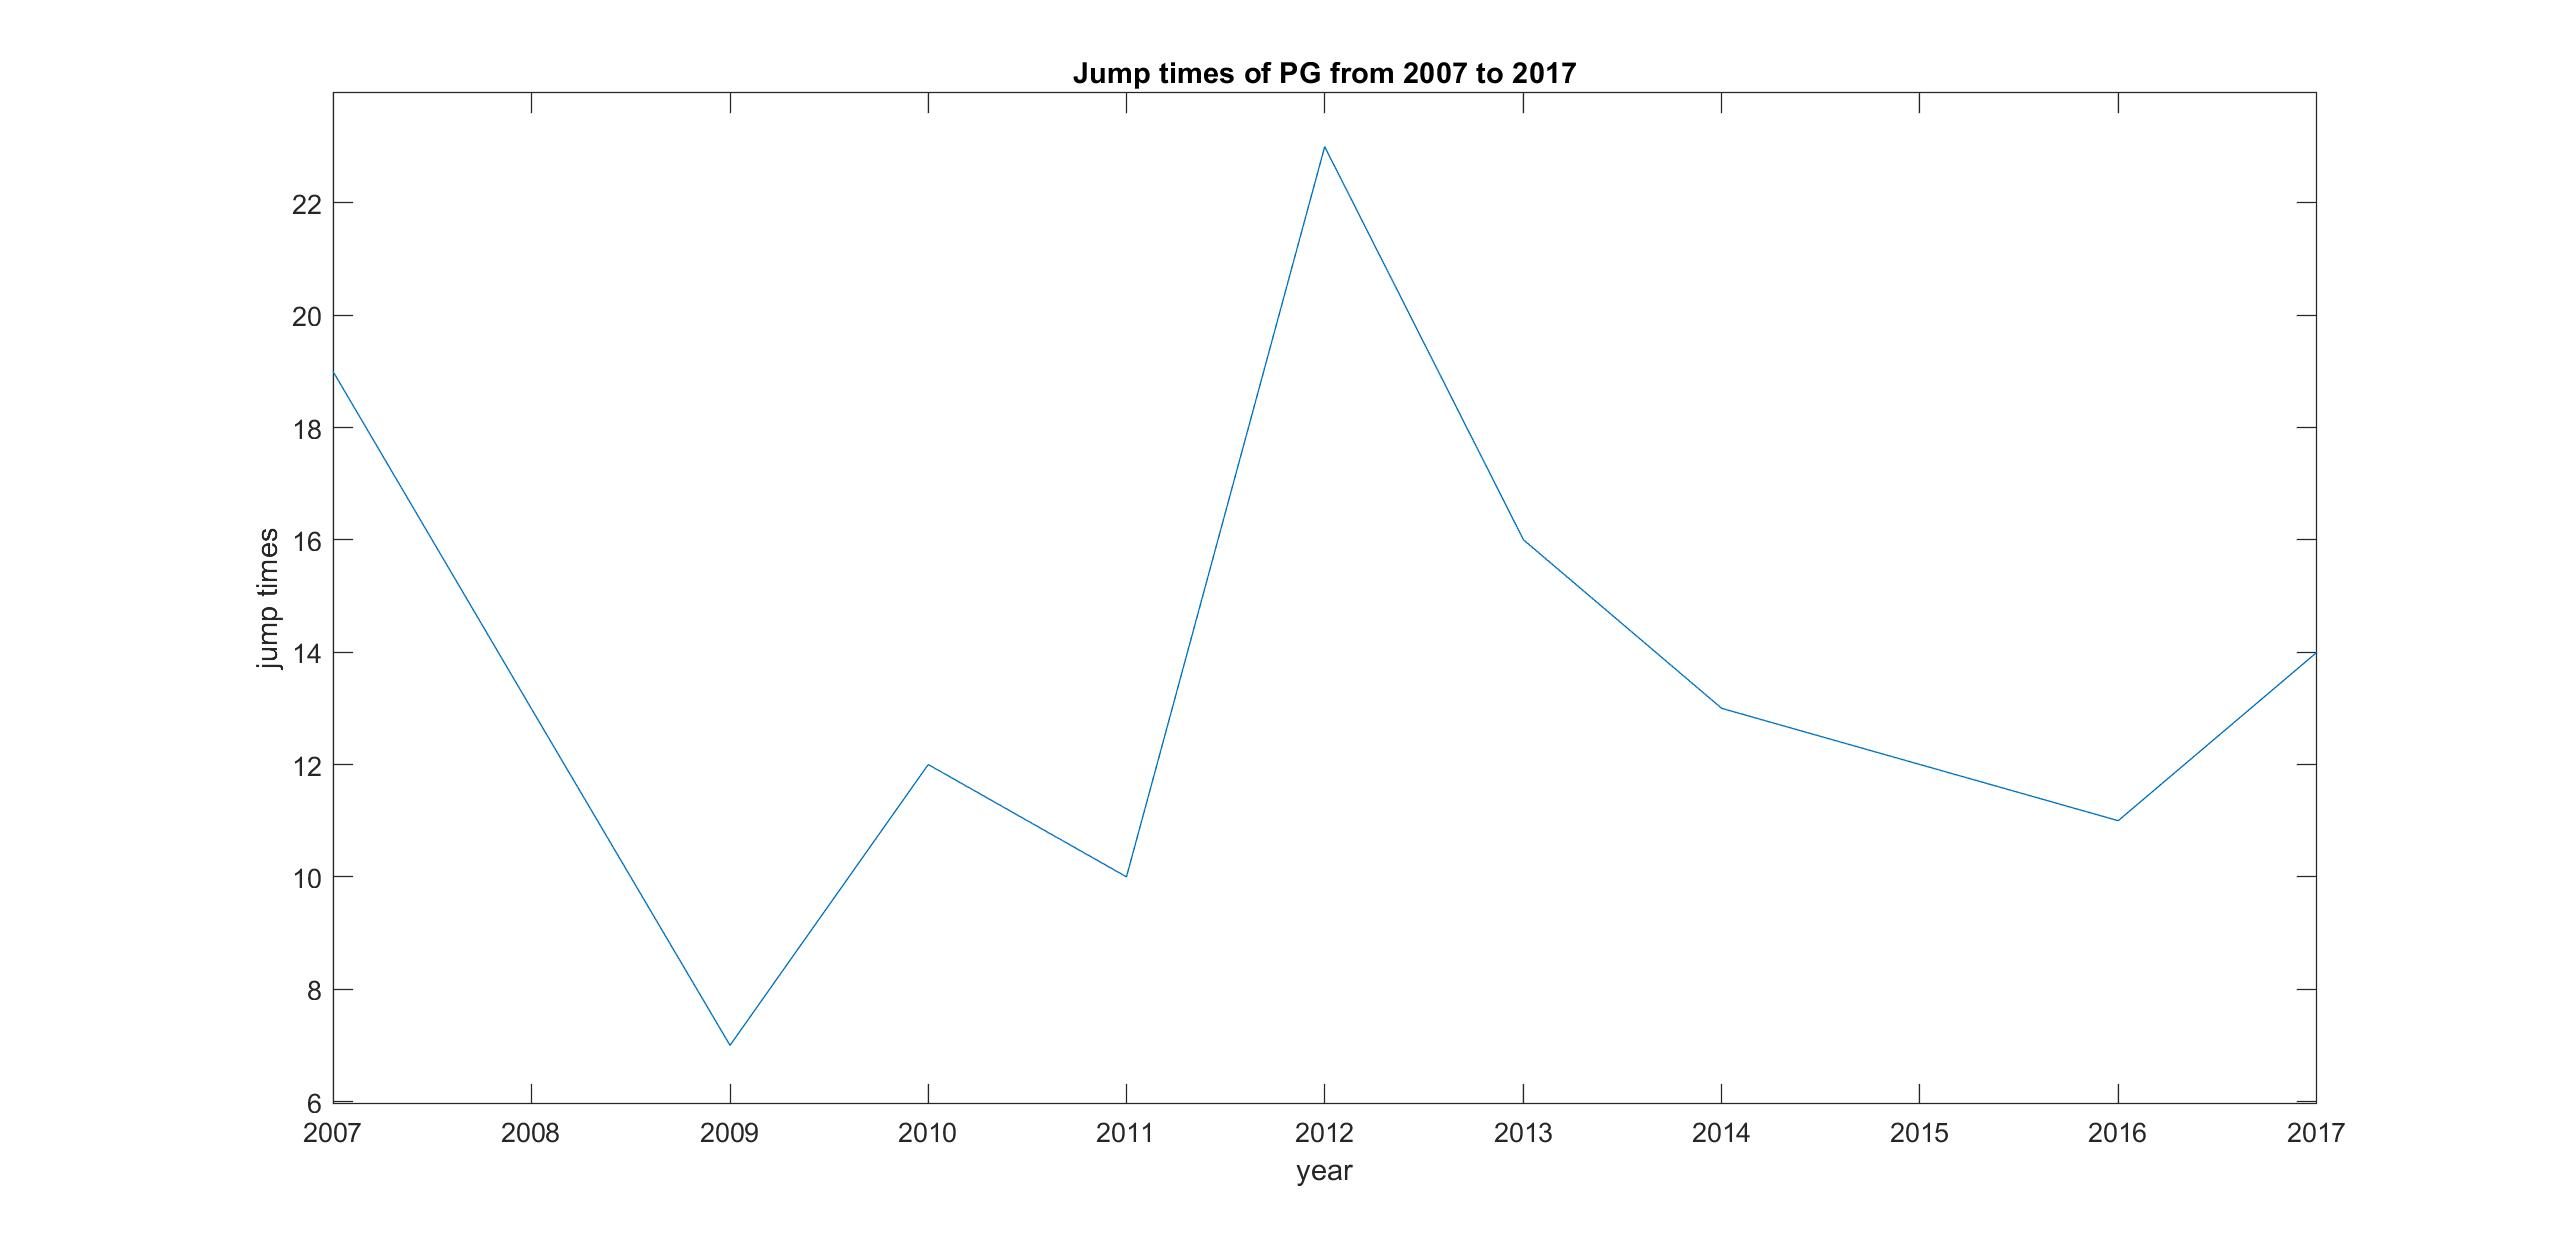
\includegraphics[width=3in]{figures/p4_ex1_a1.jpg}
            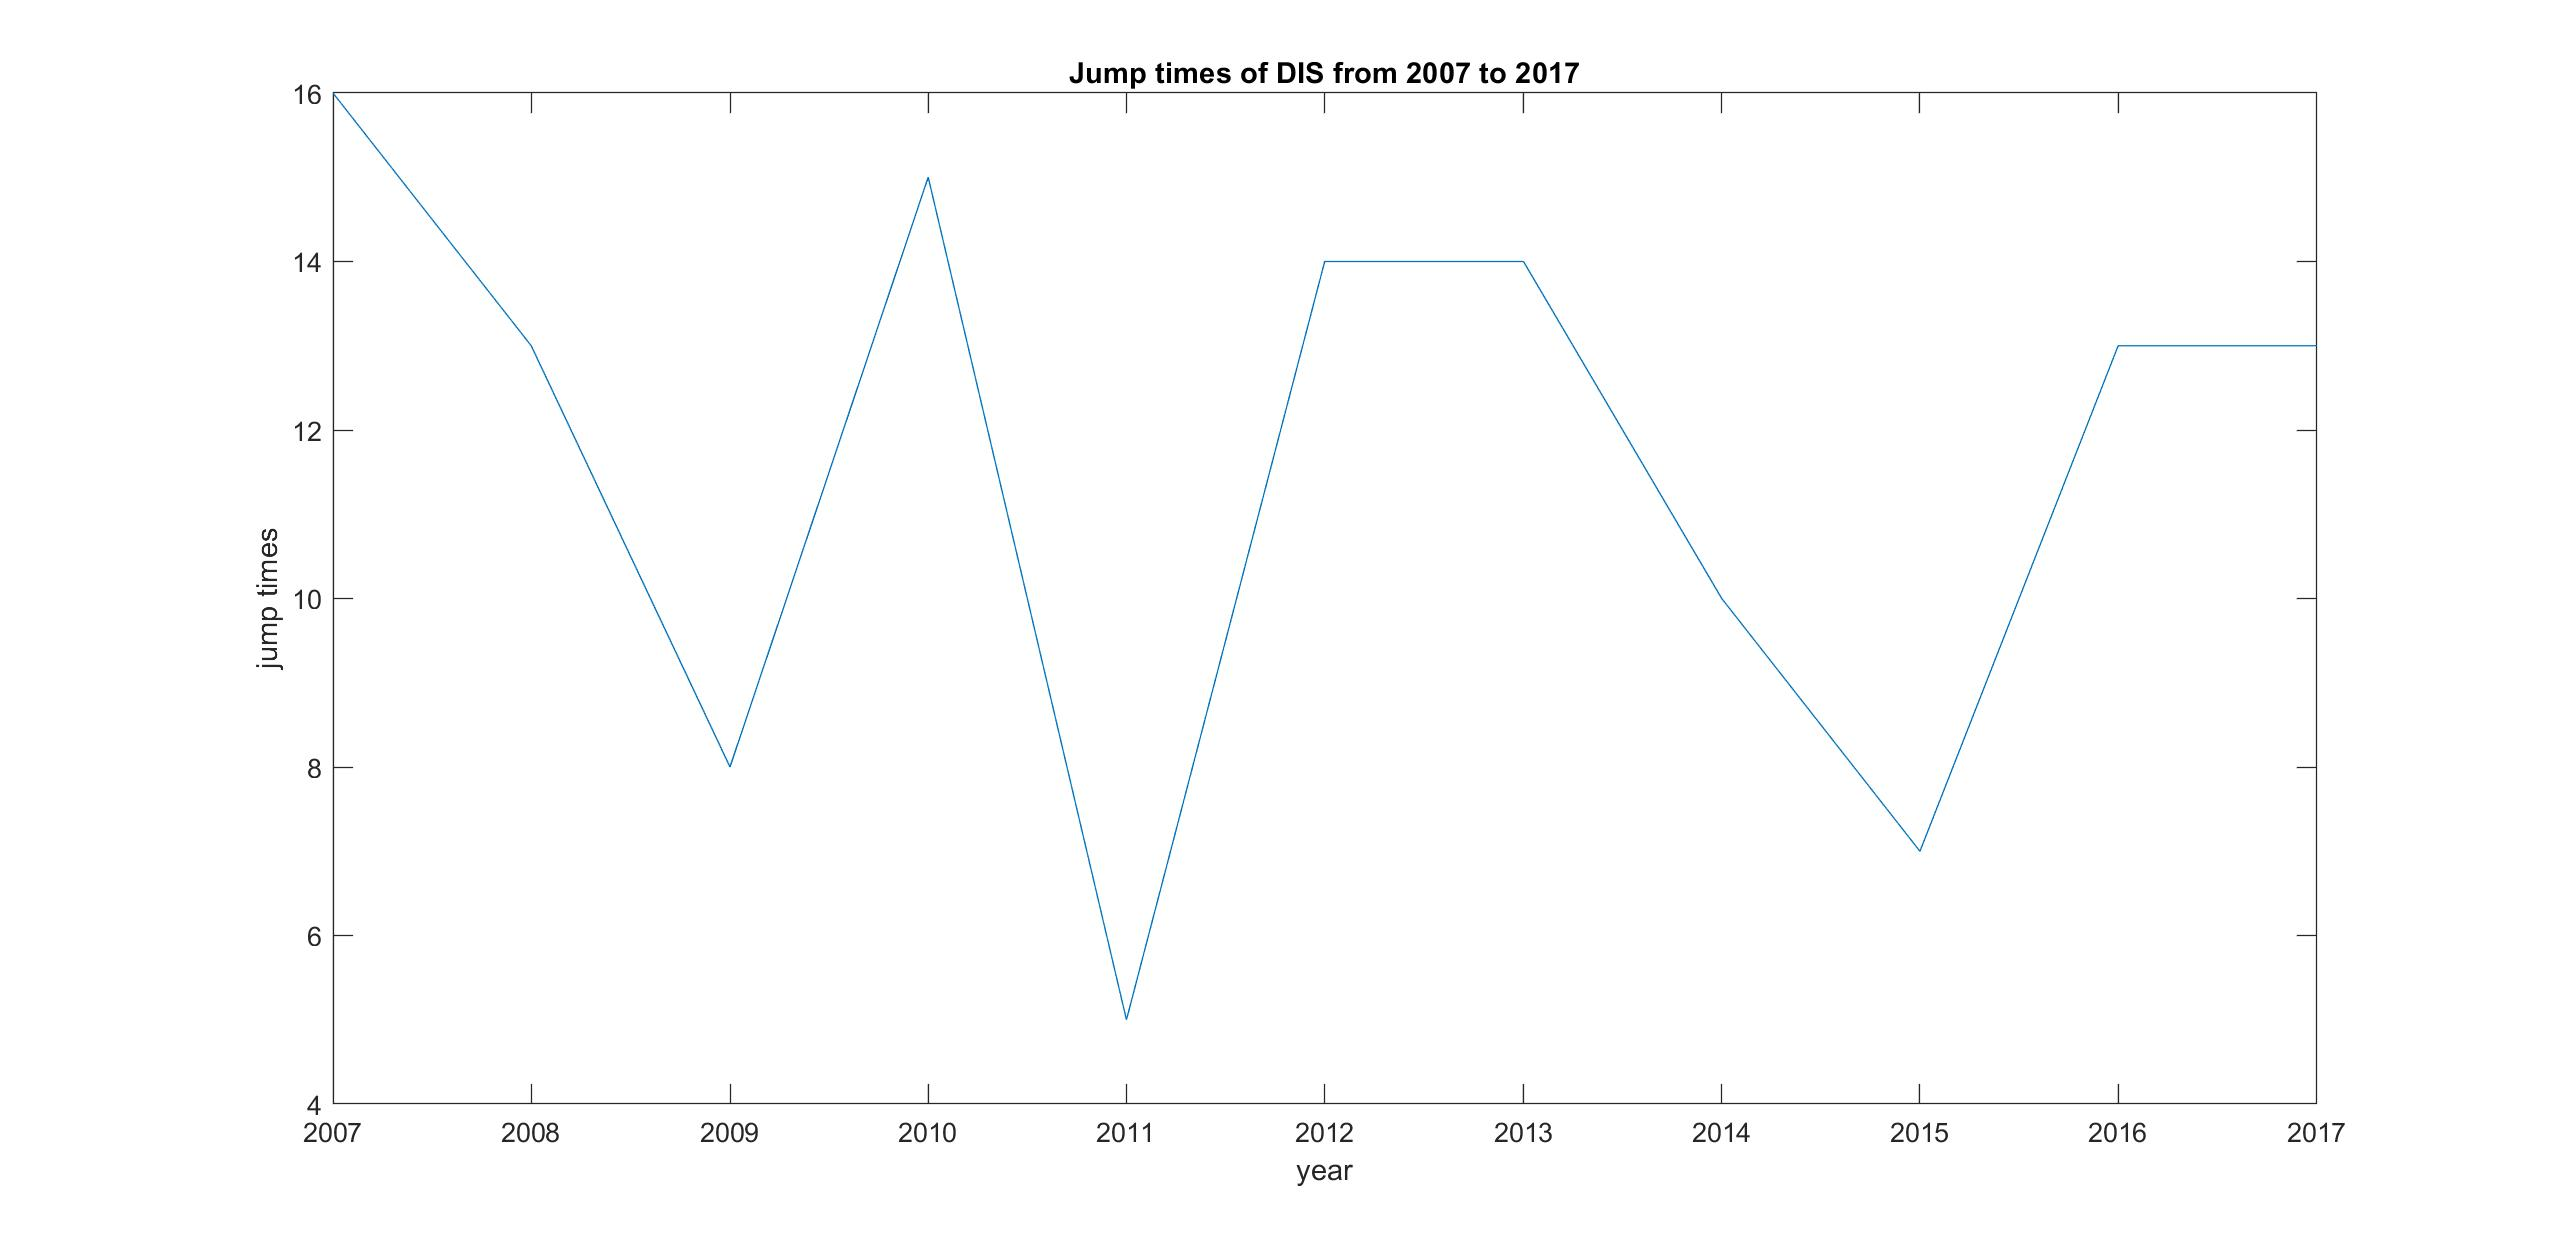
\includegraphics[width=3in]{figures/p4_ex1_a1_DIS.jpg}
            \end{minipage}
            }
            \centering
            \caption{Jumps number of PG and DIS from 2007 to 2017}
\end{figure}



%-----B-----
\item Here are the plots of truncated variance of PG and DIS in the first 2 week of 2007.

 \begin{figure}[H]
           \subfigure{
           \begin{minipage}[l]{1\linewidth}
           \centering
            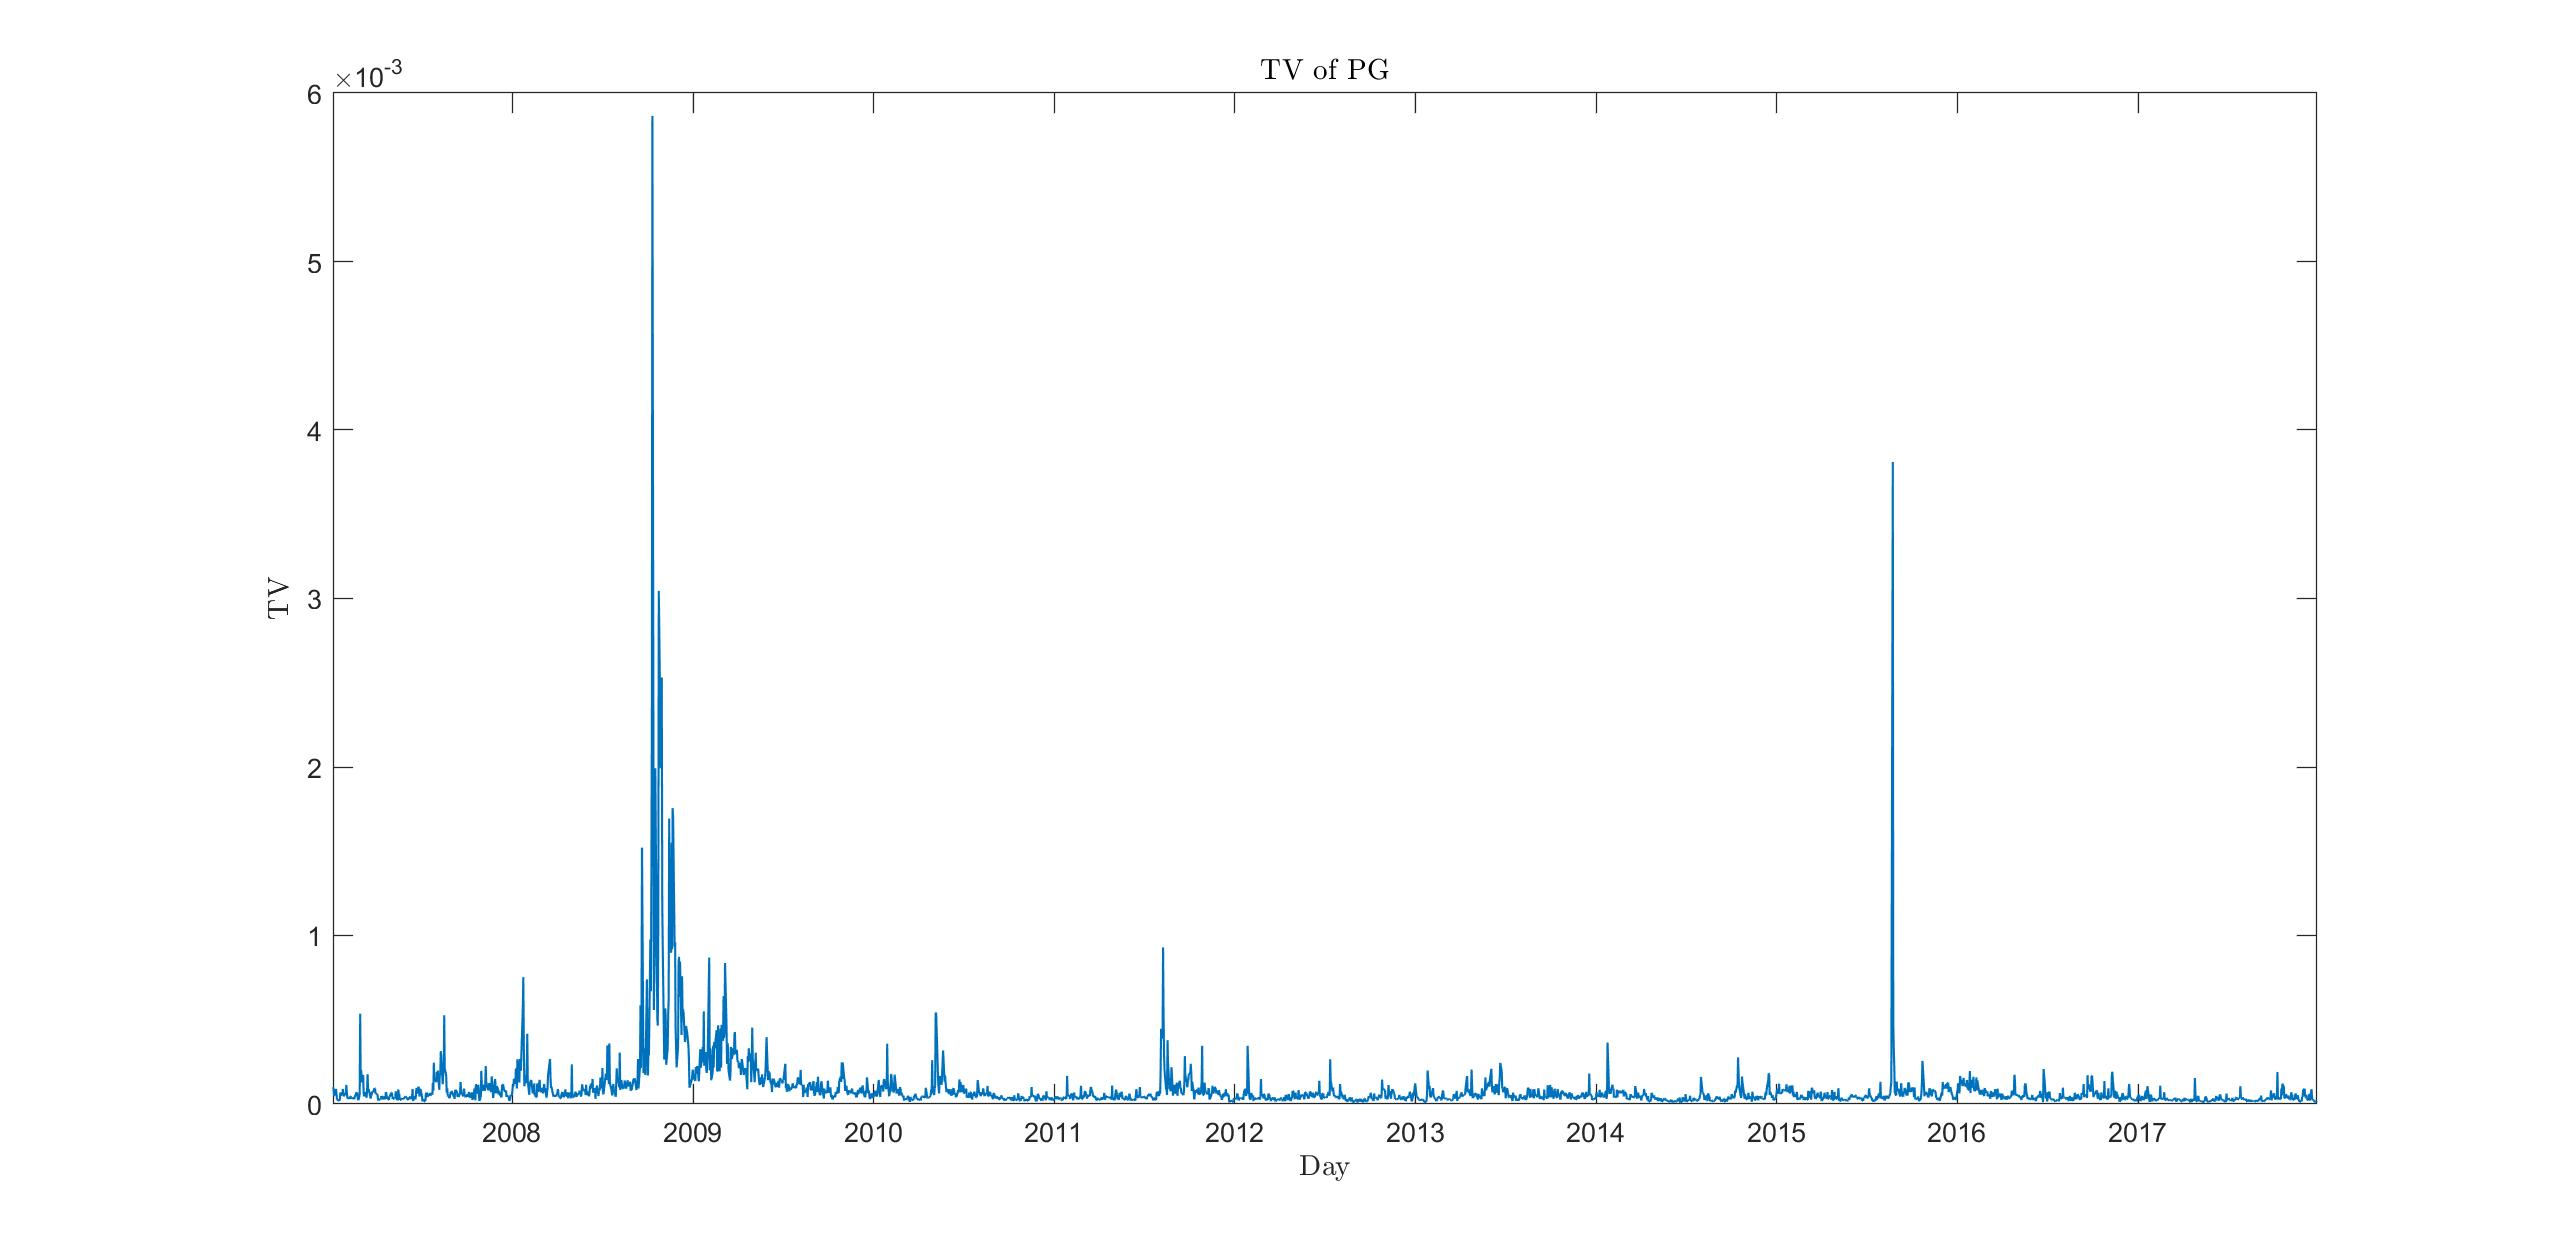
\includegraphics[width=3in]{figures/p4_ex1_b.jpg}
            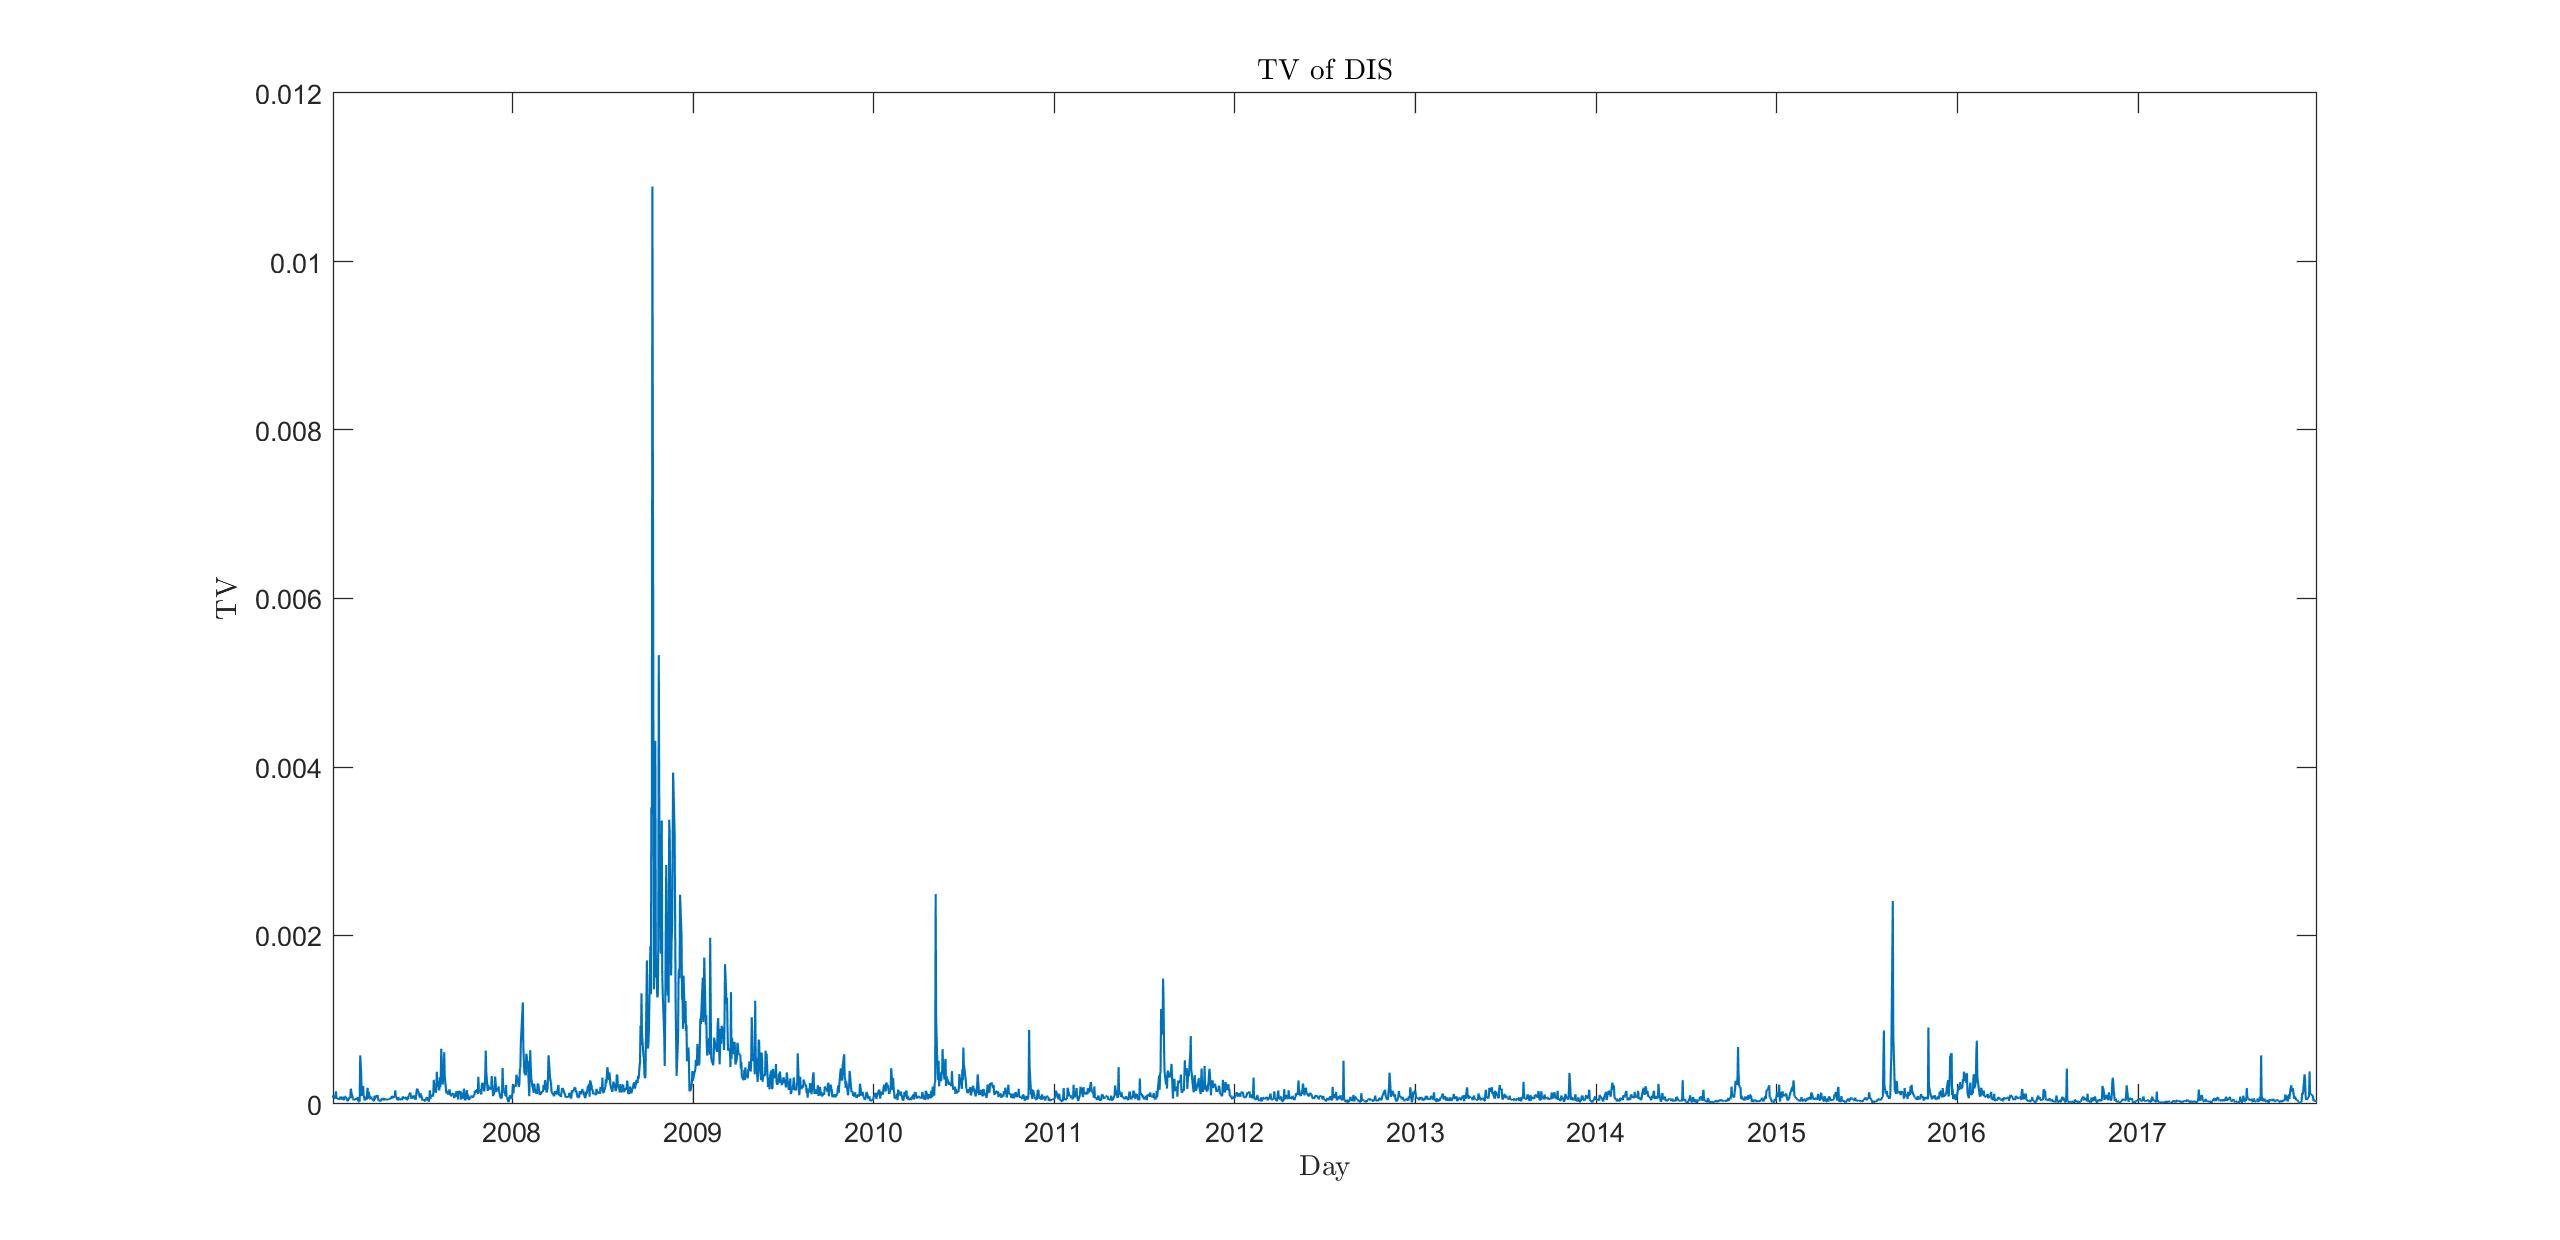
\includegraphics[width=3in]{figures/p4_ex1_b_DIS.jpg}
            \end{minipage}
            }
            \centering
            \caption{Truncated variance of PG and DIS}
\end{figure}

From this figure we can see that, the value of TV is largest around 2009, which means the stock price in 2009 has experienced a large volatility. 


%---------c-----
\item The follows are the figures of TV and estimated confidence interval of PG and DIS for the first 2 week in 2007.
 \begin{figure}[H]
           \subfigure{
           \begin{minipage}[l]{1\linewidth}
           \centering
            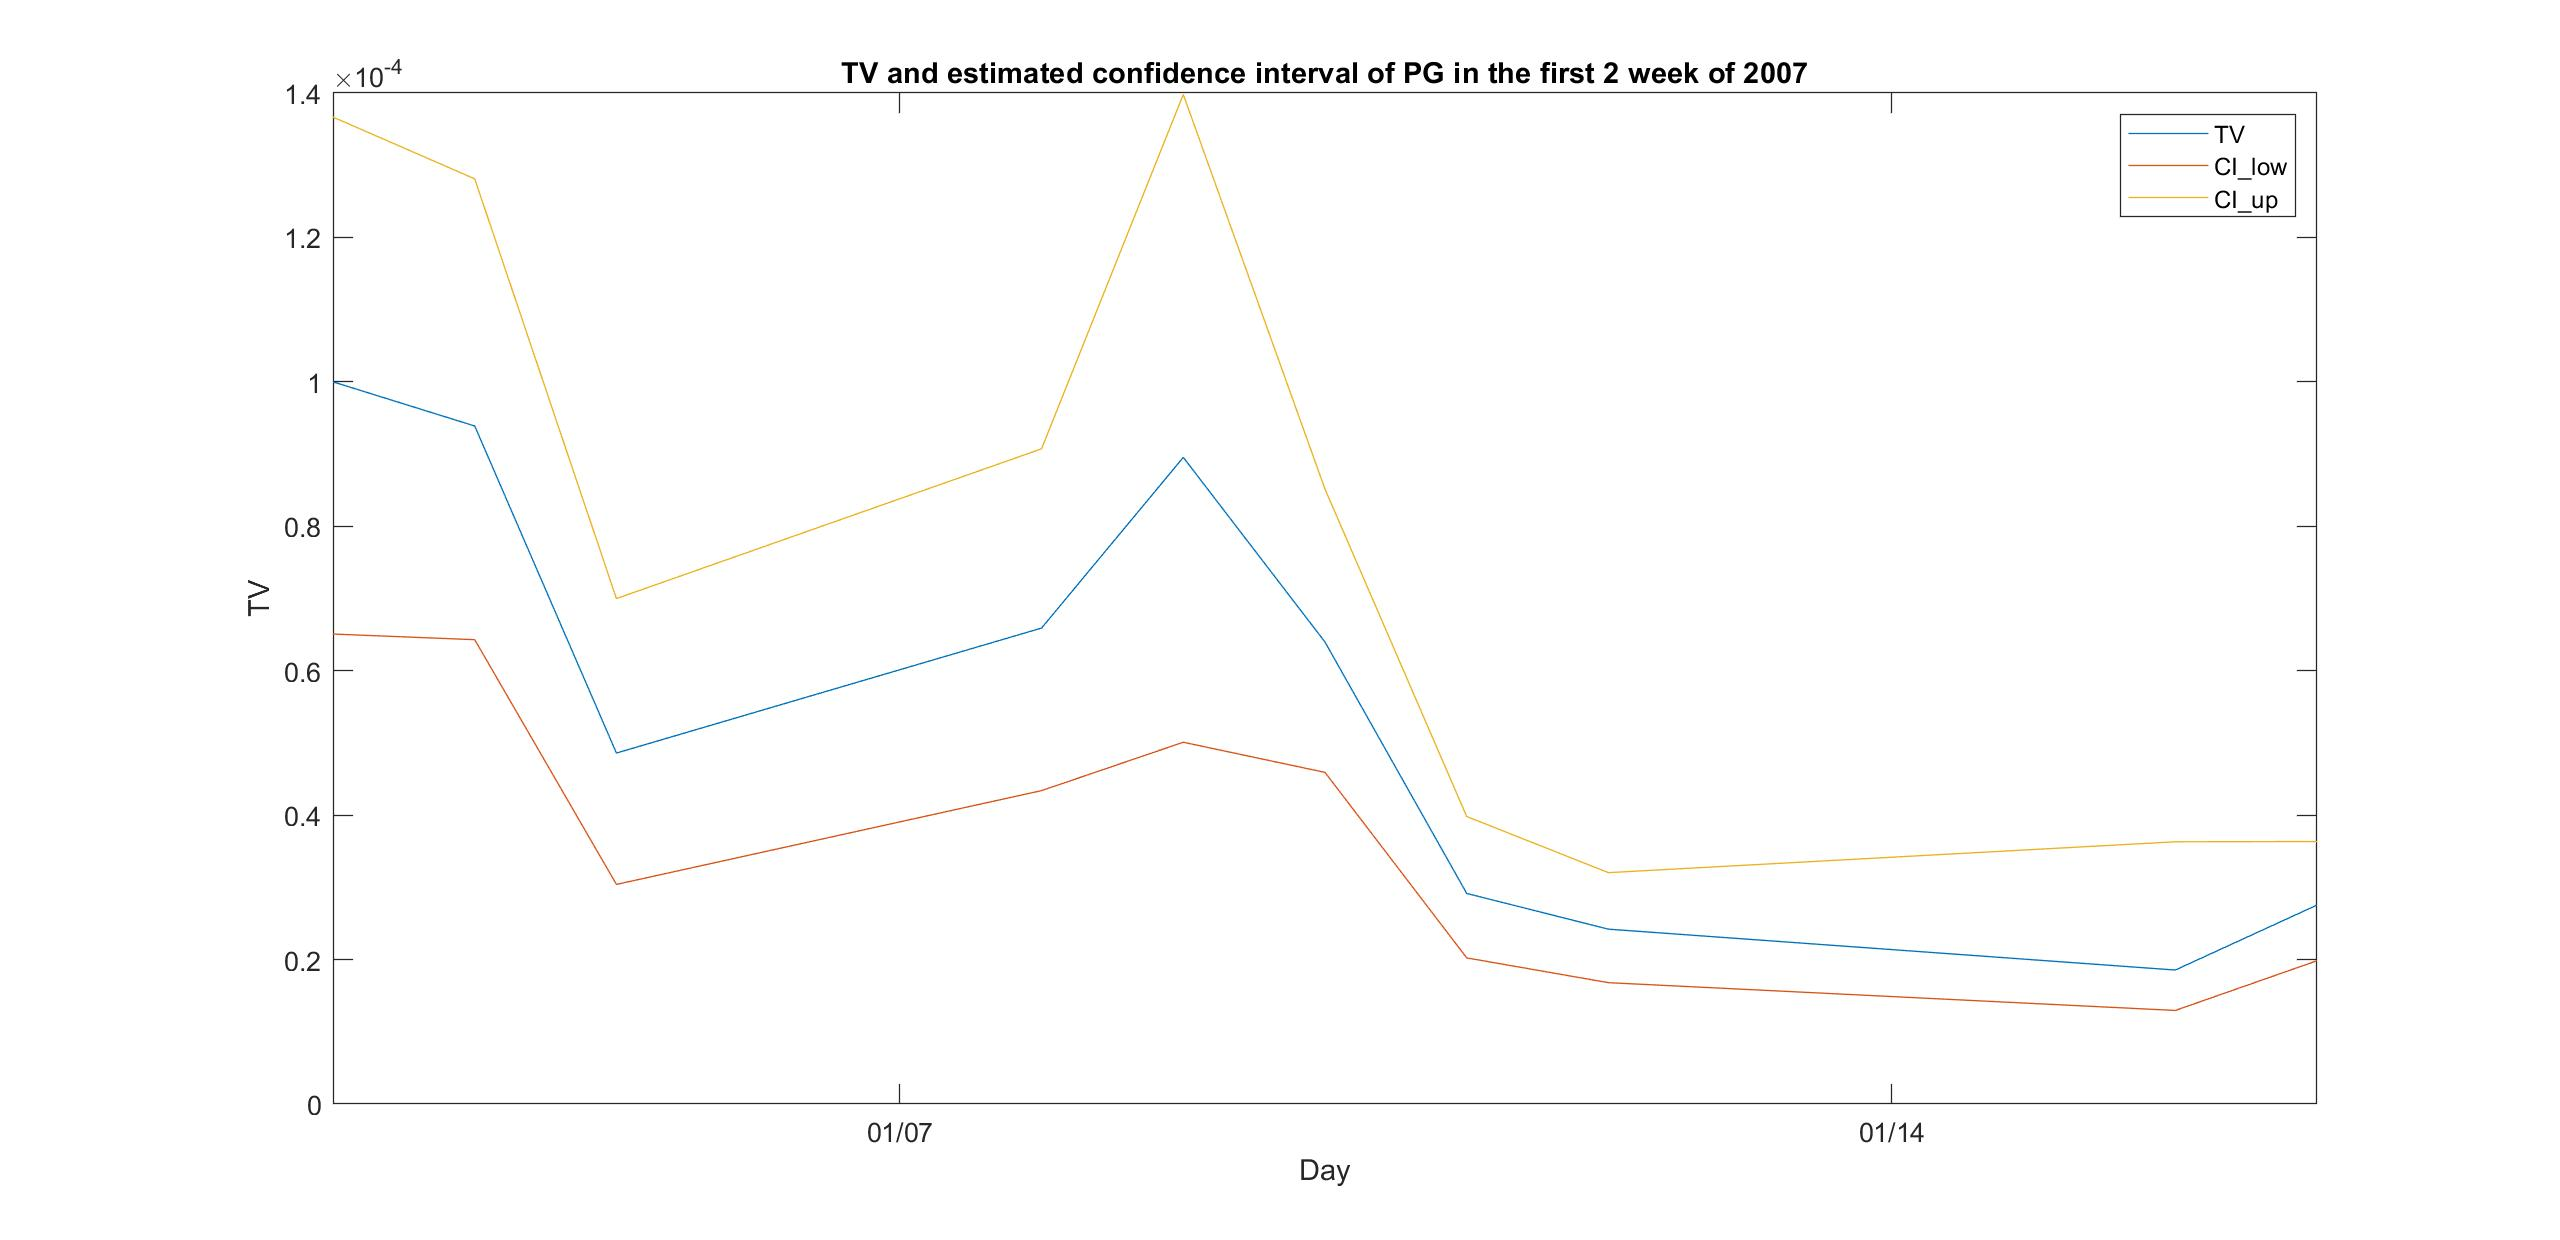
\includegraphics[width=3in]{figures/p4_ex1_c1.jpg}
            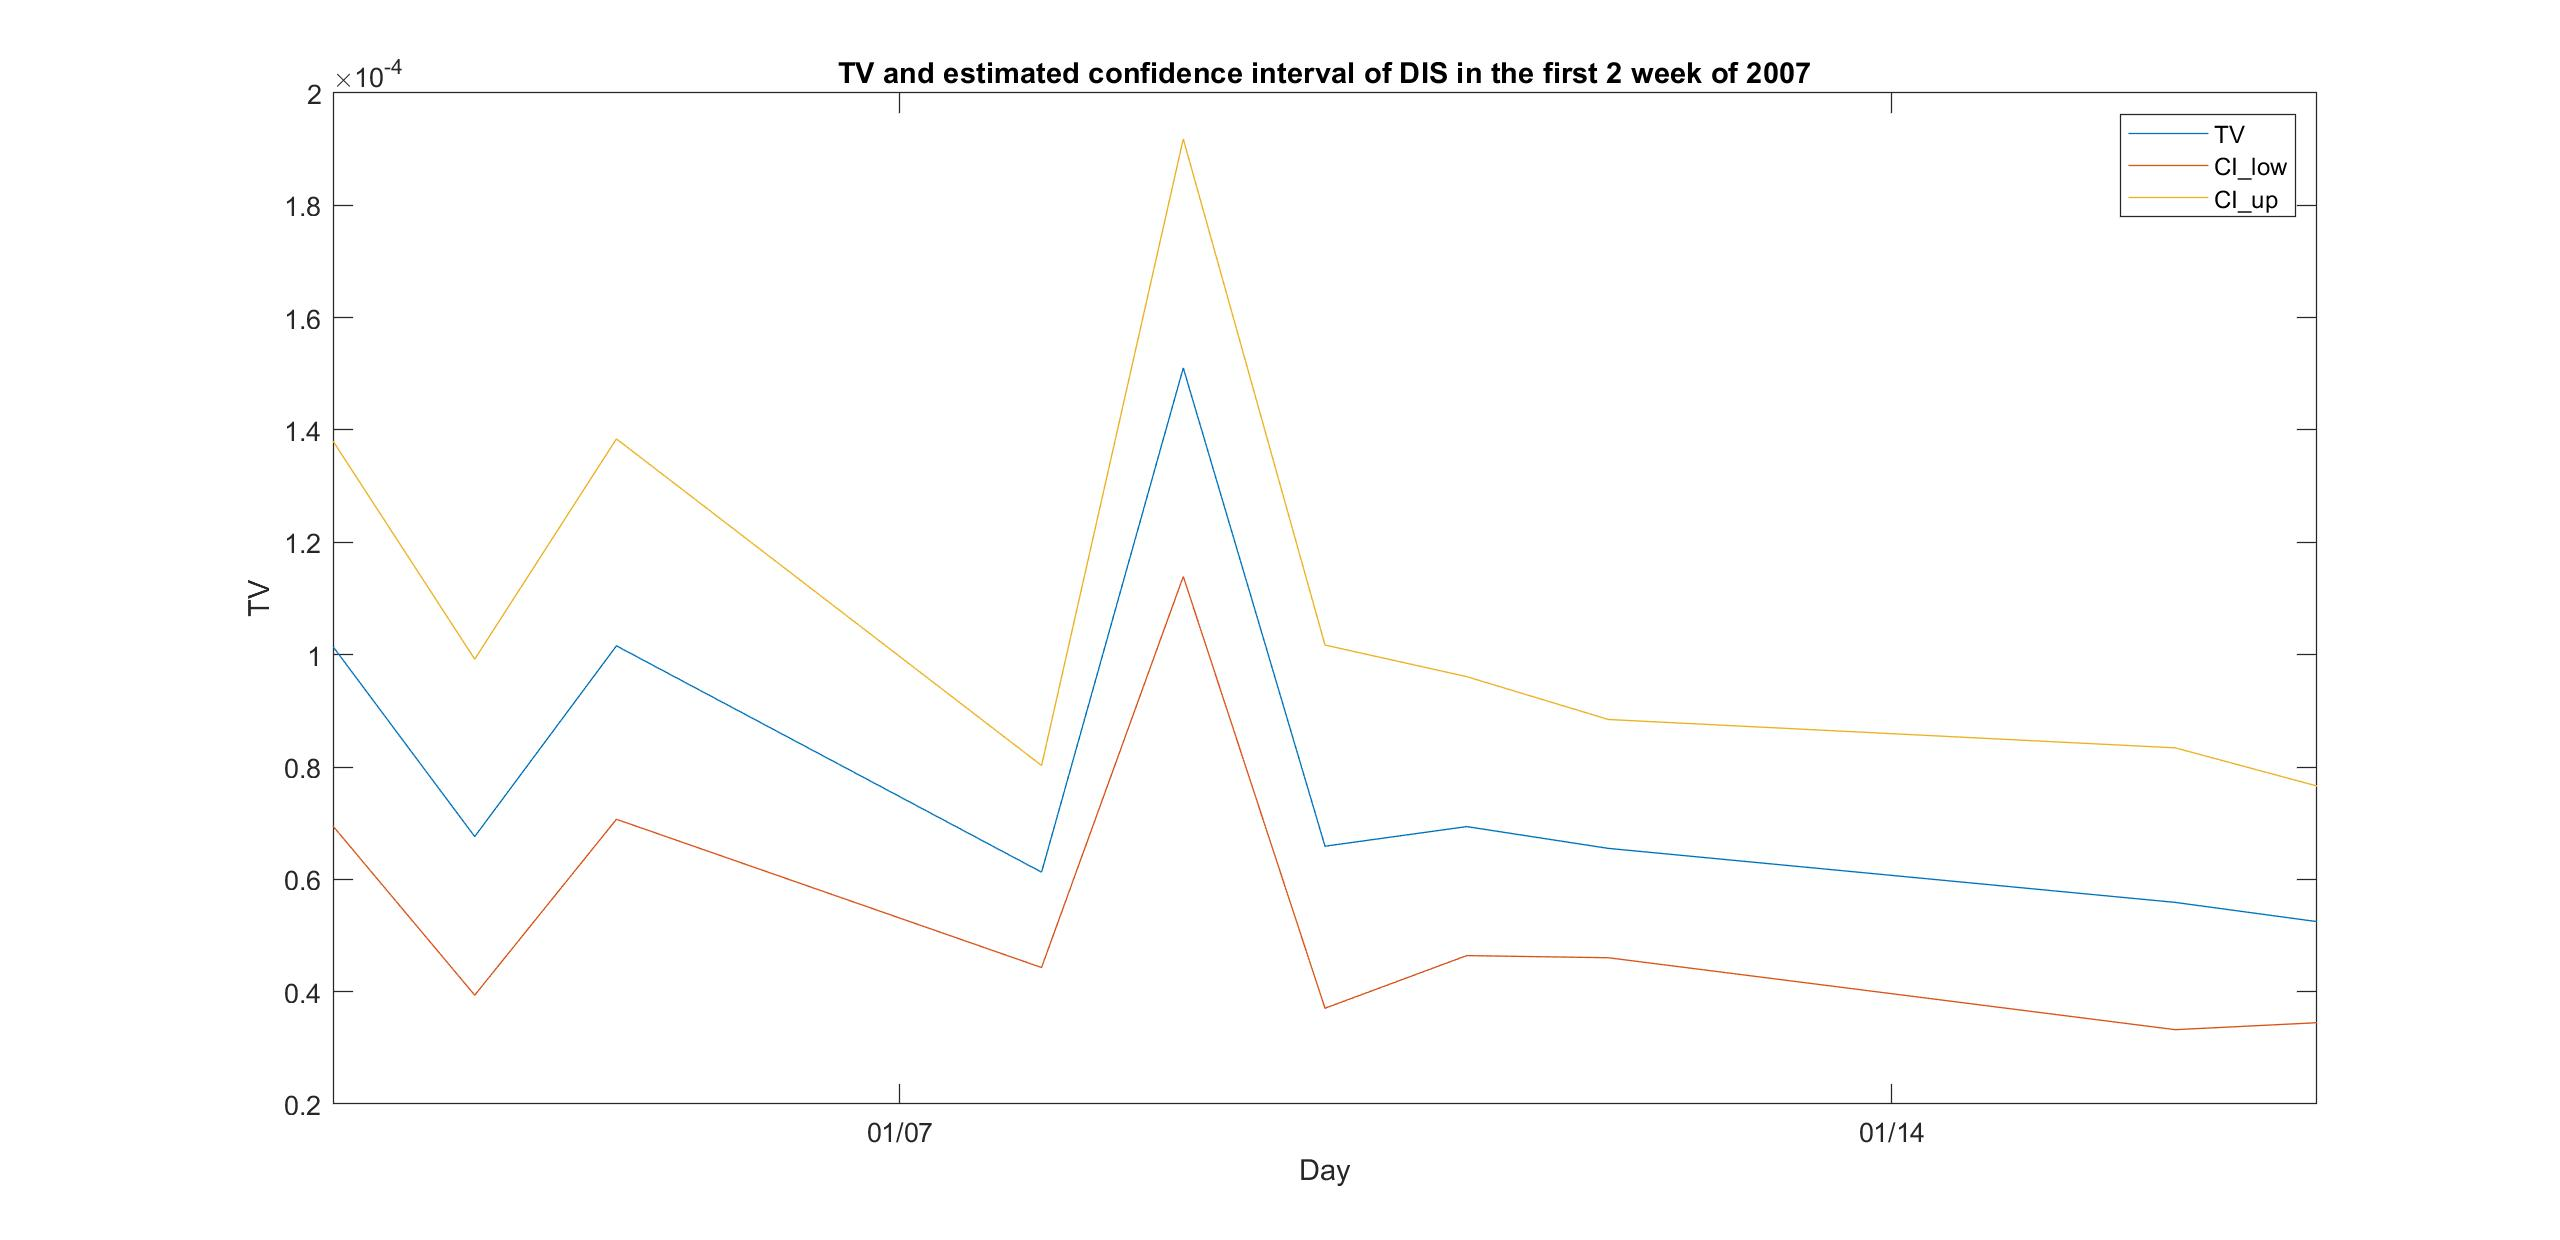
\includegraphics[width=3in]{figures/p4_ex1_c1_DIS.jpg}
            \end{minipage}
            }
            \centering
            \caption{Truncated variance and confidence interval of PG and DIS (first 2 week of 2007)}
\end{figure}

The range of TV for PG and DIS are (0.2$\times10^{-4}$,1.0 $\times10^{-4}$) and (0.5 $\times10^{-4}$,1.6 $\times10^{-4}$) respectively. According to the range of TV we can see that, the volatility of DIS' log returns' volatility is bigger that PG's, which means that the risk of DIS may be higher than PG's.  We can also see that around January 10, the value of both PG and DIS' TV have experienced a big fluctuation.

As for the estimated confidence interval, it is clear that all the value of IV are bounded by the upper confidence interval and the lower confidence interval. We can calculate the cover rate of the confidence interval for PG and DIS: the cover rate for PG is 100\% and the cover rate for DIS is 100\%. These results are better than using asymptotic distribution( in project 3).

%-------------d----------
\item We do not need to apply Delta method to compute the confidence interval of annualized integral variance. Bootstrap method calculate the confidence interval for estimators by finding the quantile of samples, since transferring daily truncated variance to annualized truncated variance is a homogeneous increasing function, the rank of sample data will not change: the 97.5\% quantile and 2.5\% quantile of annualized truncated variance is just the annualized 97.5\% quantile and 2.5\% quantile of daily truncated variance.\\

%-------------e----------
\item The follows are the figures of annualized TV and estimated confidence interval of PG and DIS for the first 2 week in 2007.

 \begin{figure}[H]
           \subfigure{
           \begin{minipage}[l]{1\linewidth}
           \centering
            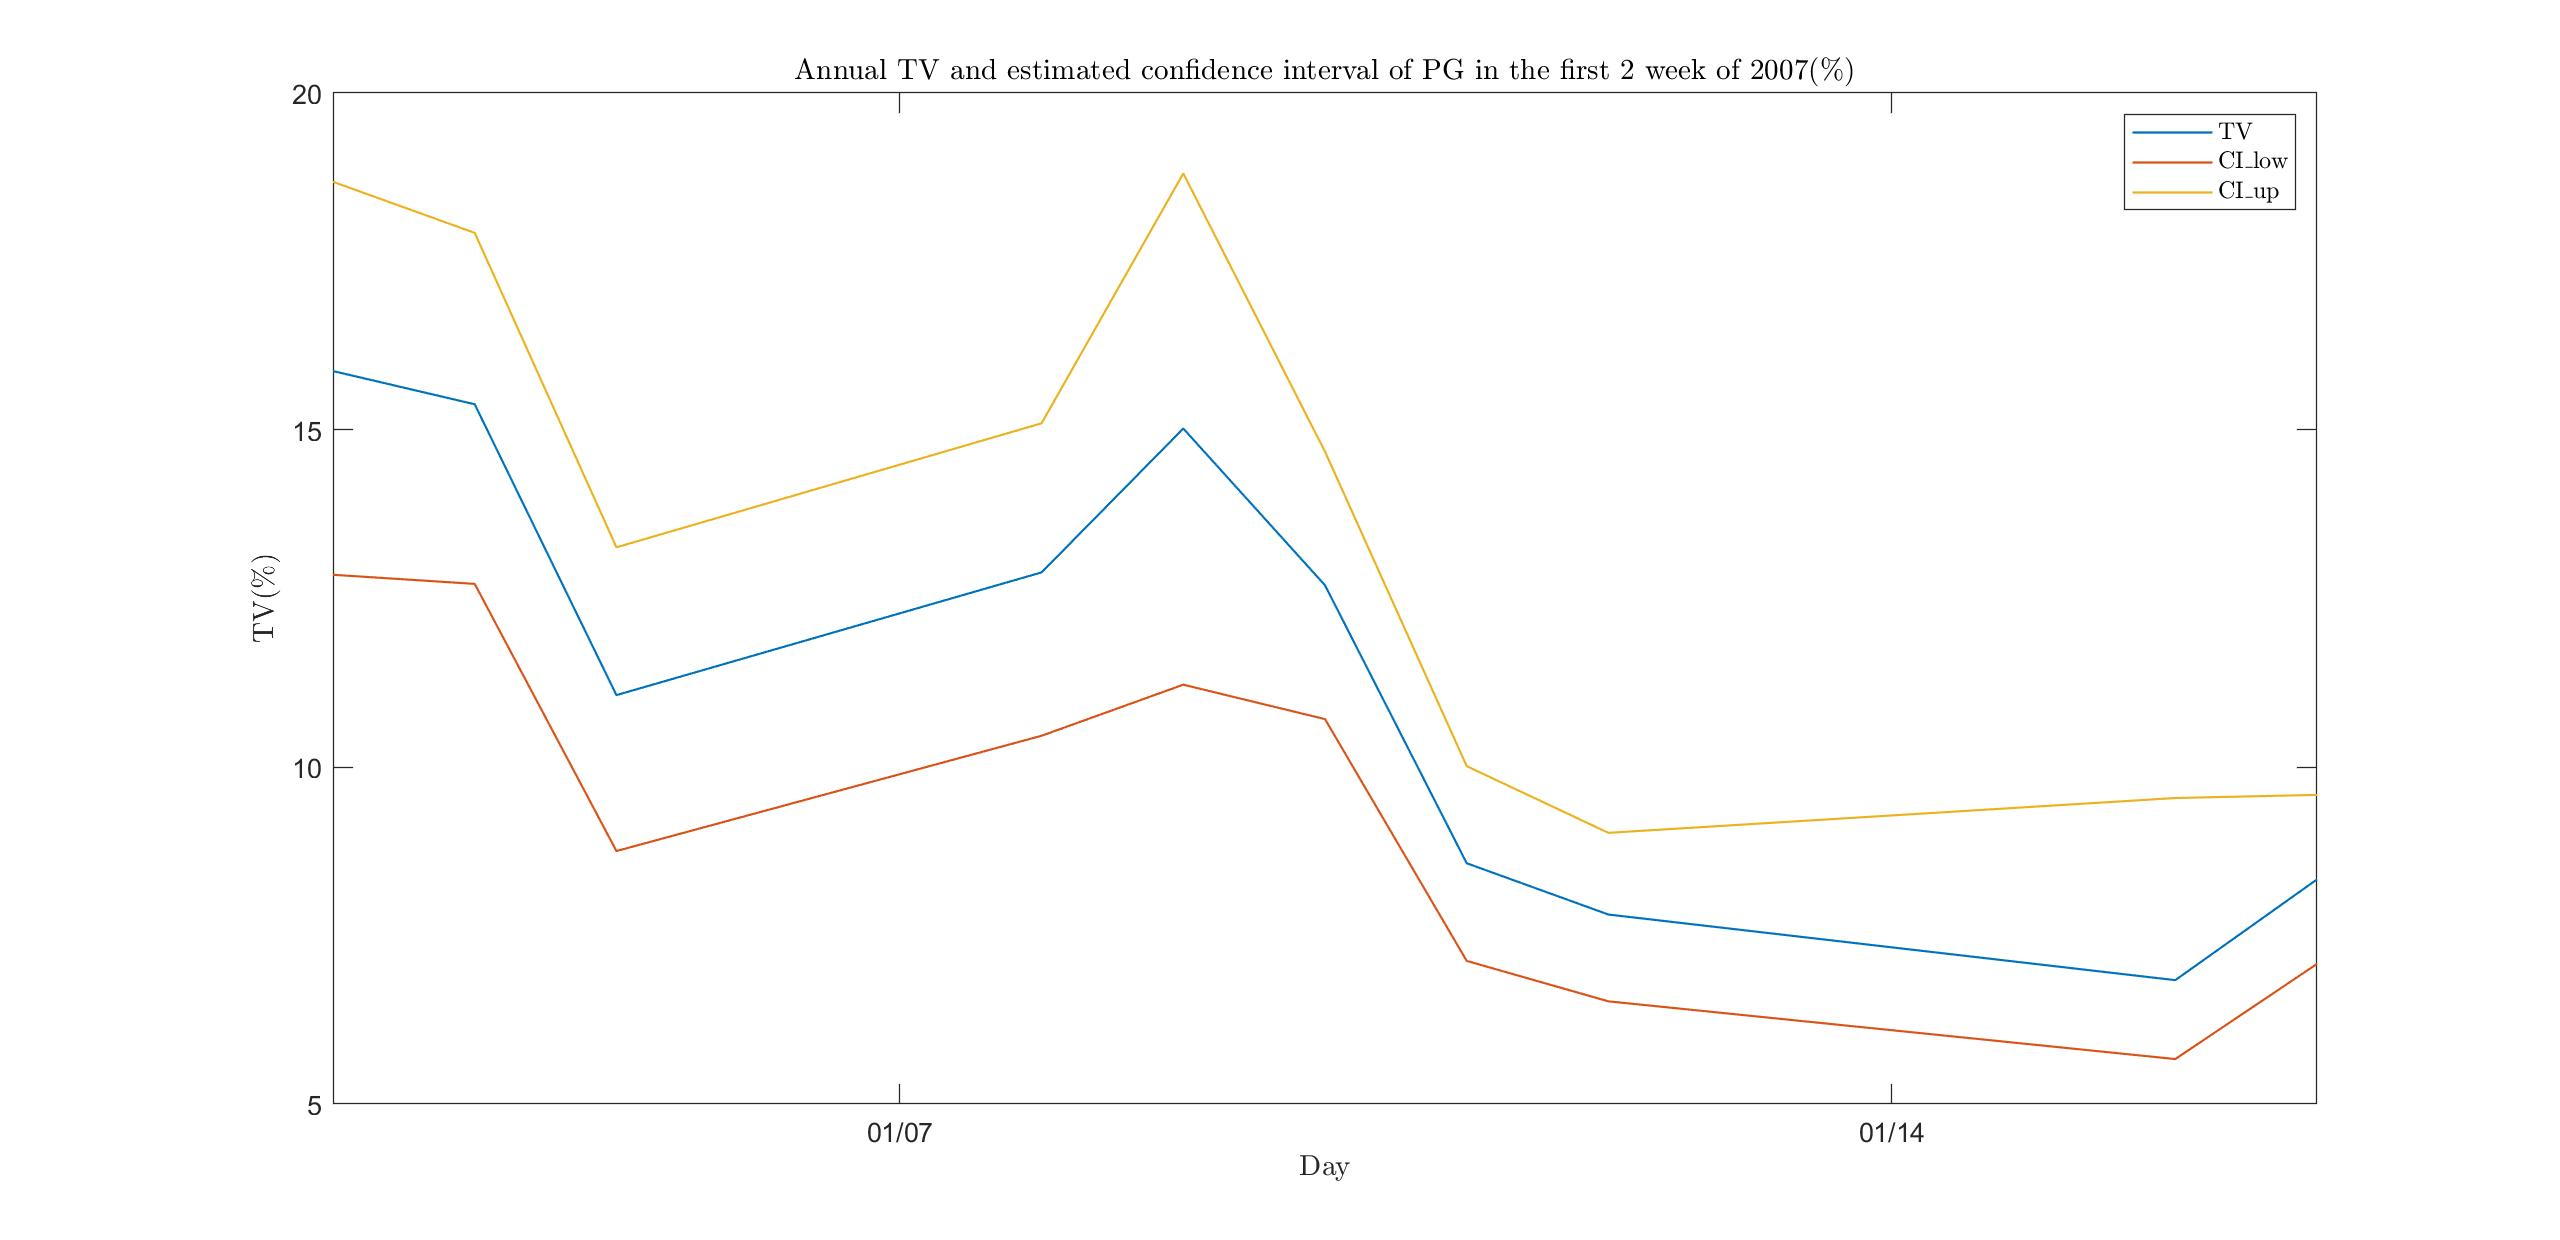
\includegraphics[width=3in]{figures/p4_ex1_e1.jpg}
            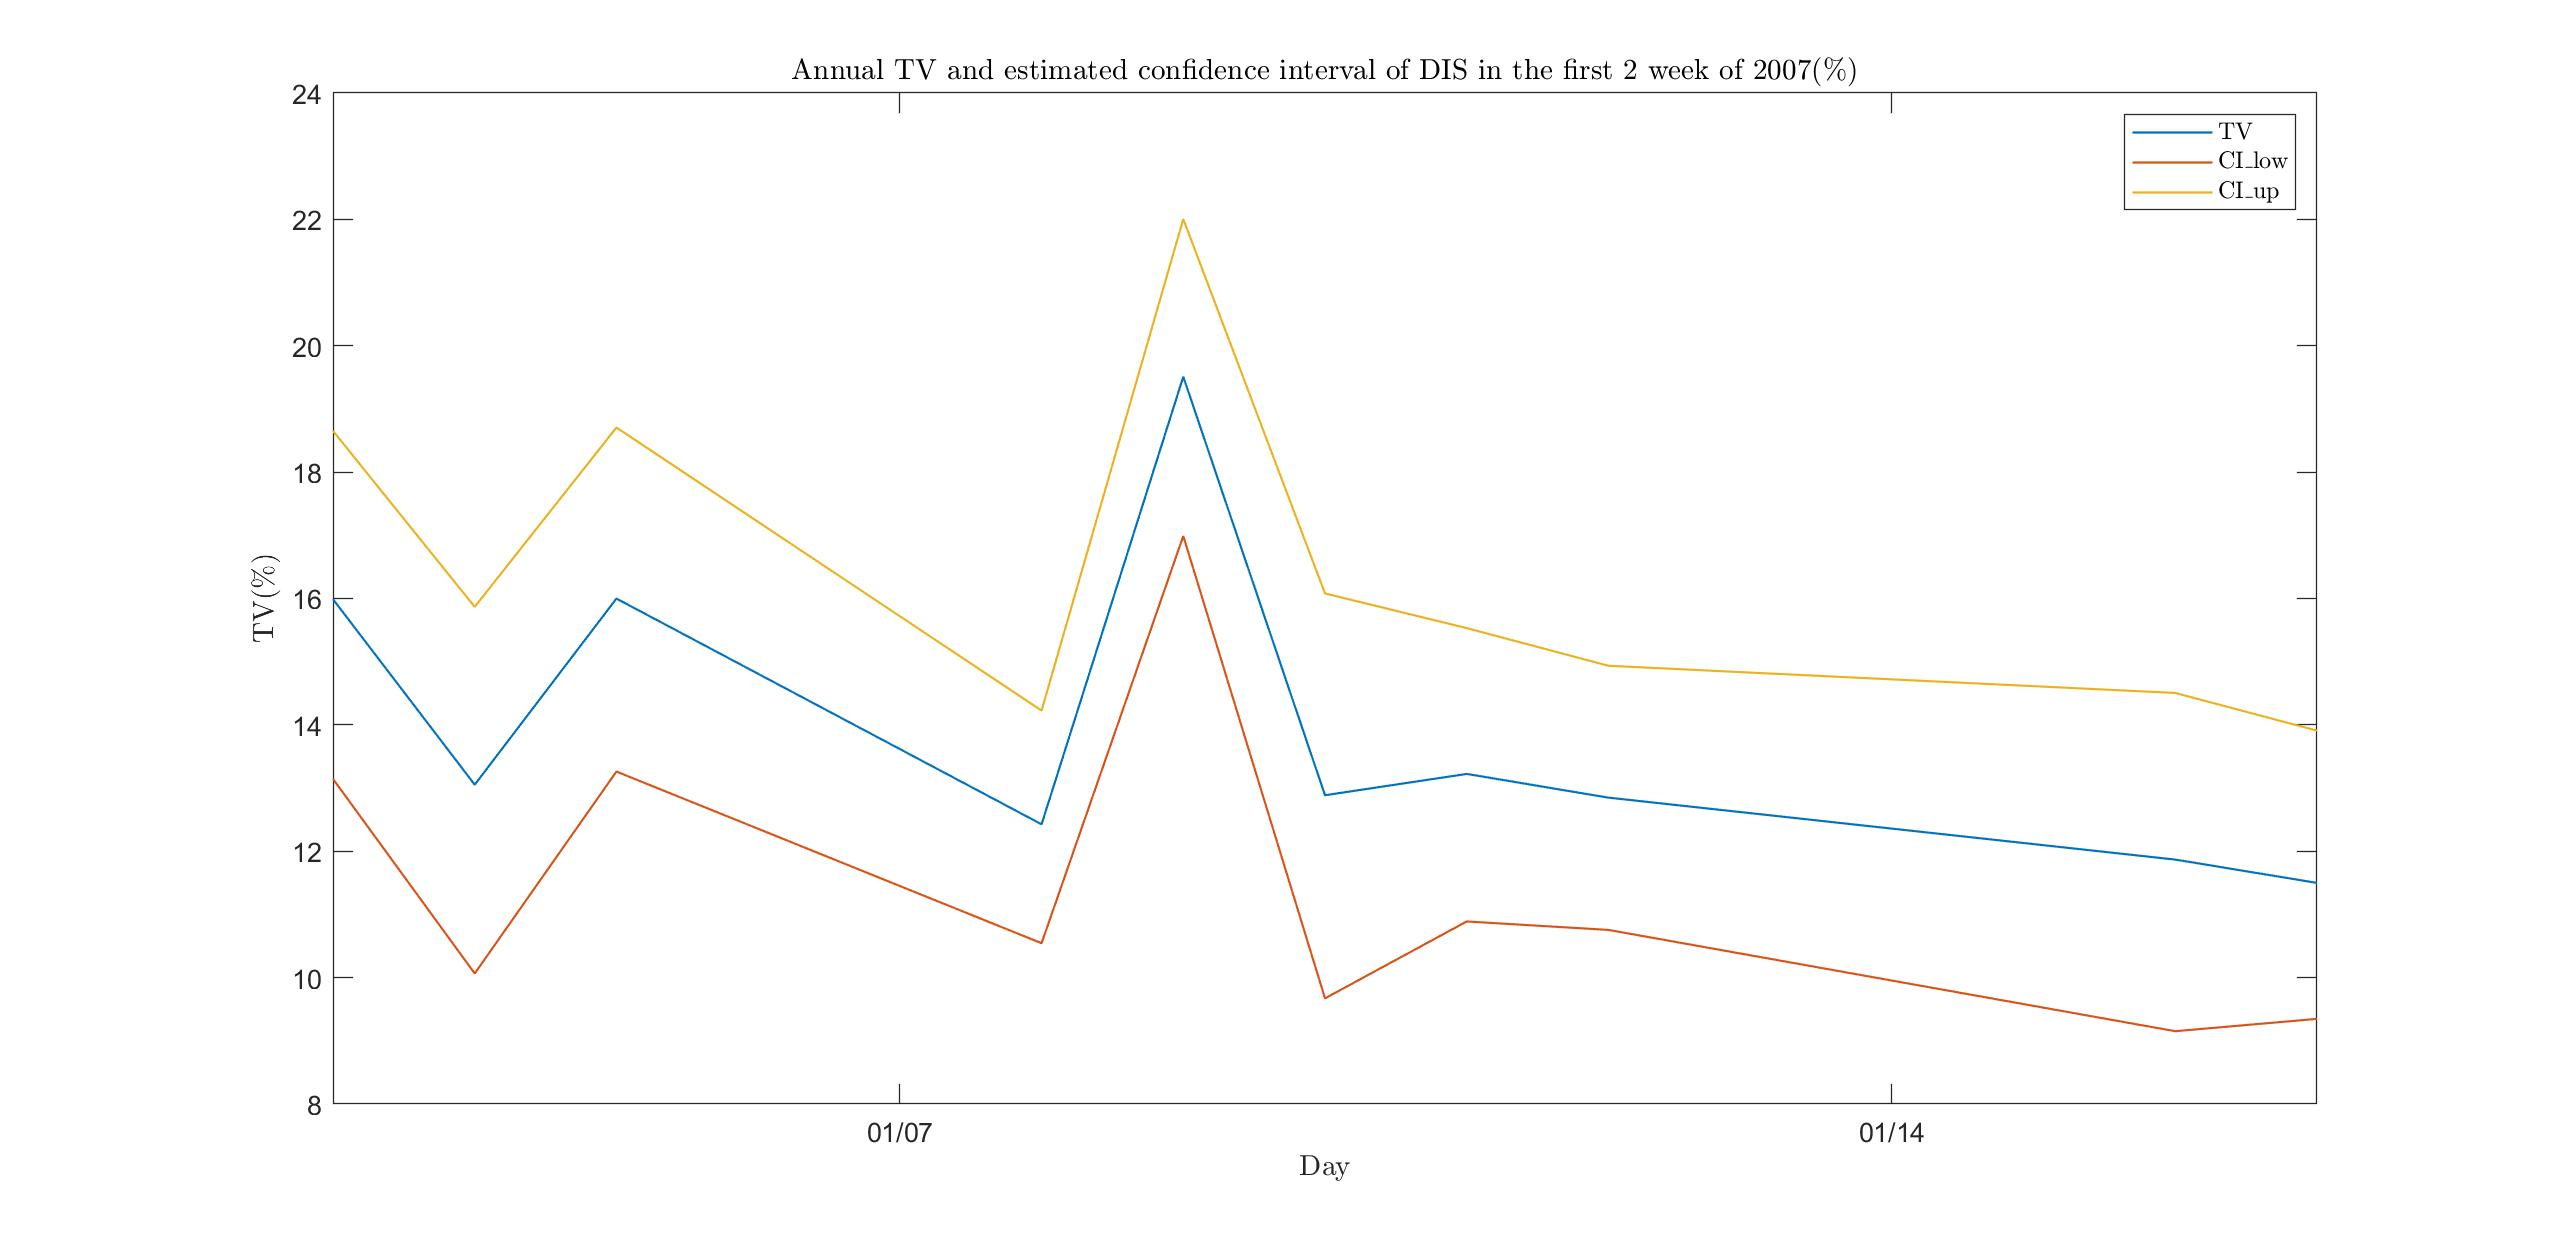
\includegraphics[width=3in]{figures/p4_ex1_e1_DIS.jpg}
            \end{minipage}
            }
            \centering
            \caption{Annualized truncated variance and confidence interval of PG and DIS (first 2 week of 2007)}
\end{figure}

The range of annual TV for PG and DIS are (5\%, 12\%) and (11\%, 20\%) respectively. For the estimated confidence interval, we can find that all the value of IV are bounded by the confidence interval. We can calculate the cover rate of the confidence interval for annual PG and DIS' TV: the cover rate for PG is 100\% and the cover rate for DIS is 100\%. These results are the same as what we find in part C. According to the result, we can verify that when calculate annual TV's confidence interval, we can first transfer daily sample base into annualized data, and use the new data to do bootstrap (we do not need to use delta method). 


%------f-----
\item The follows are the figures of IV and confidence interval estimated by asymptotic distribution and bootstrap method.
 \begin{figure}[H]
           \subfigure{
           \begin{minipage}[l]{1\linewidth}
           \centering
            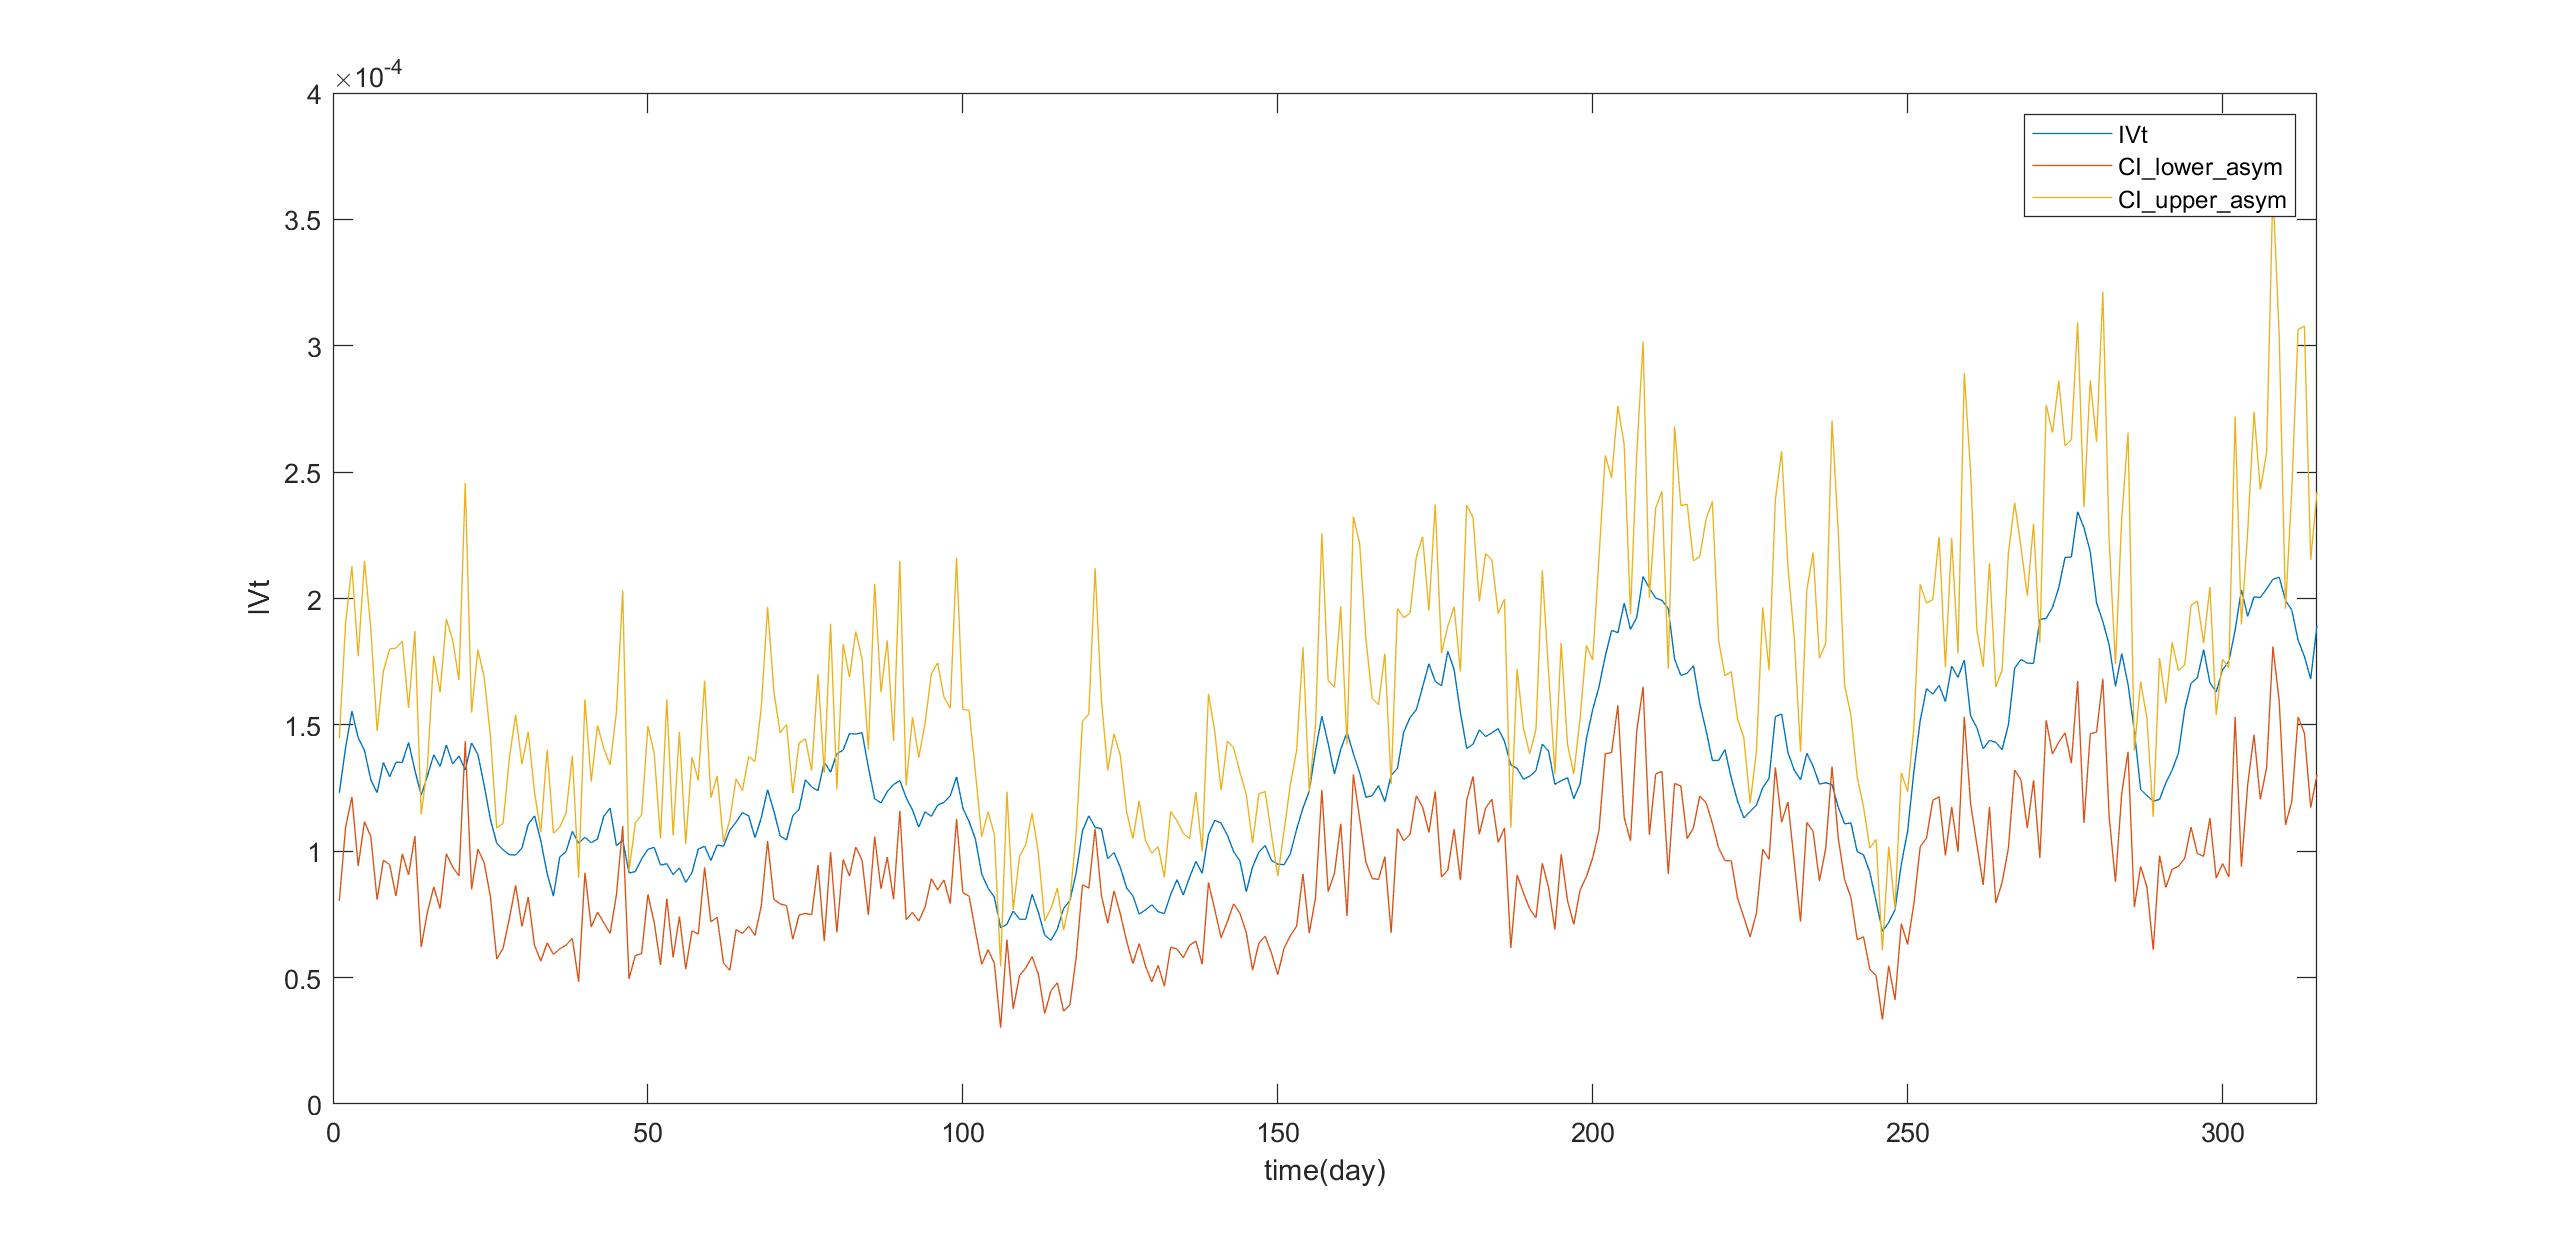
\includegraphics[width=3in]{figures/p4_ex1_f_as.jpg}
            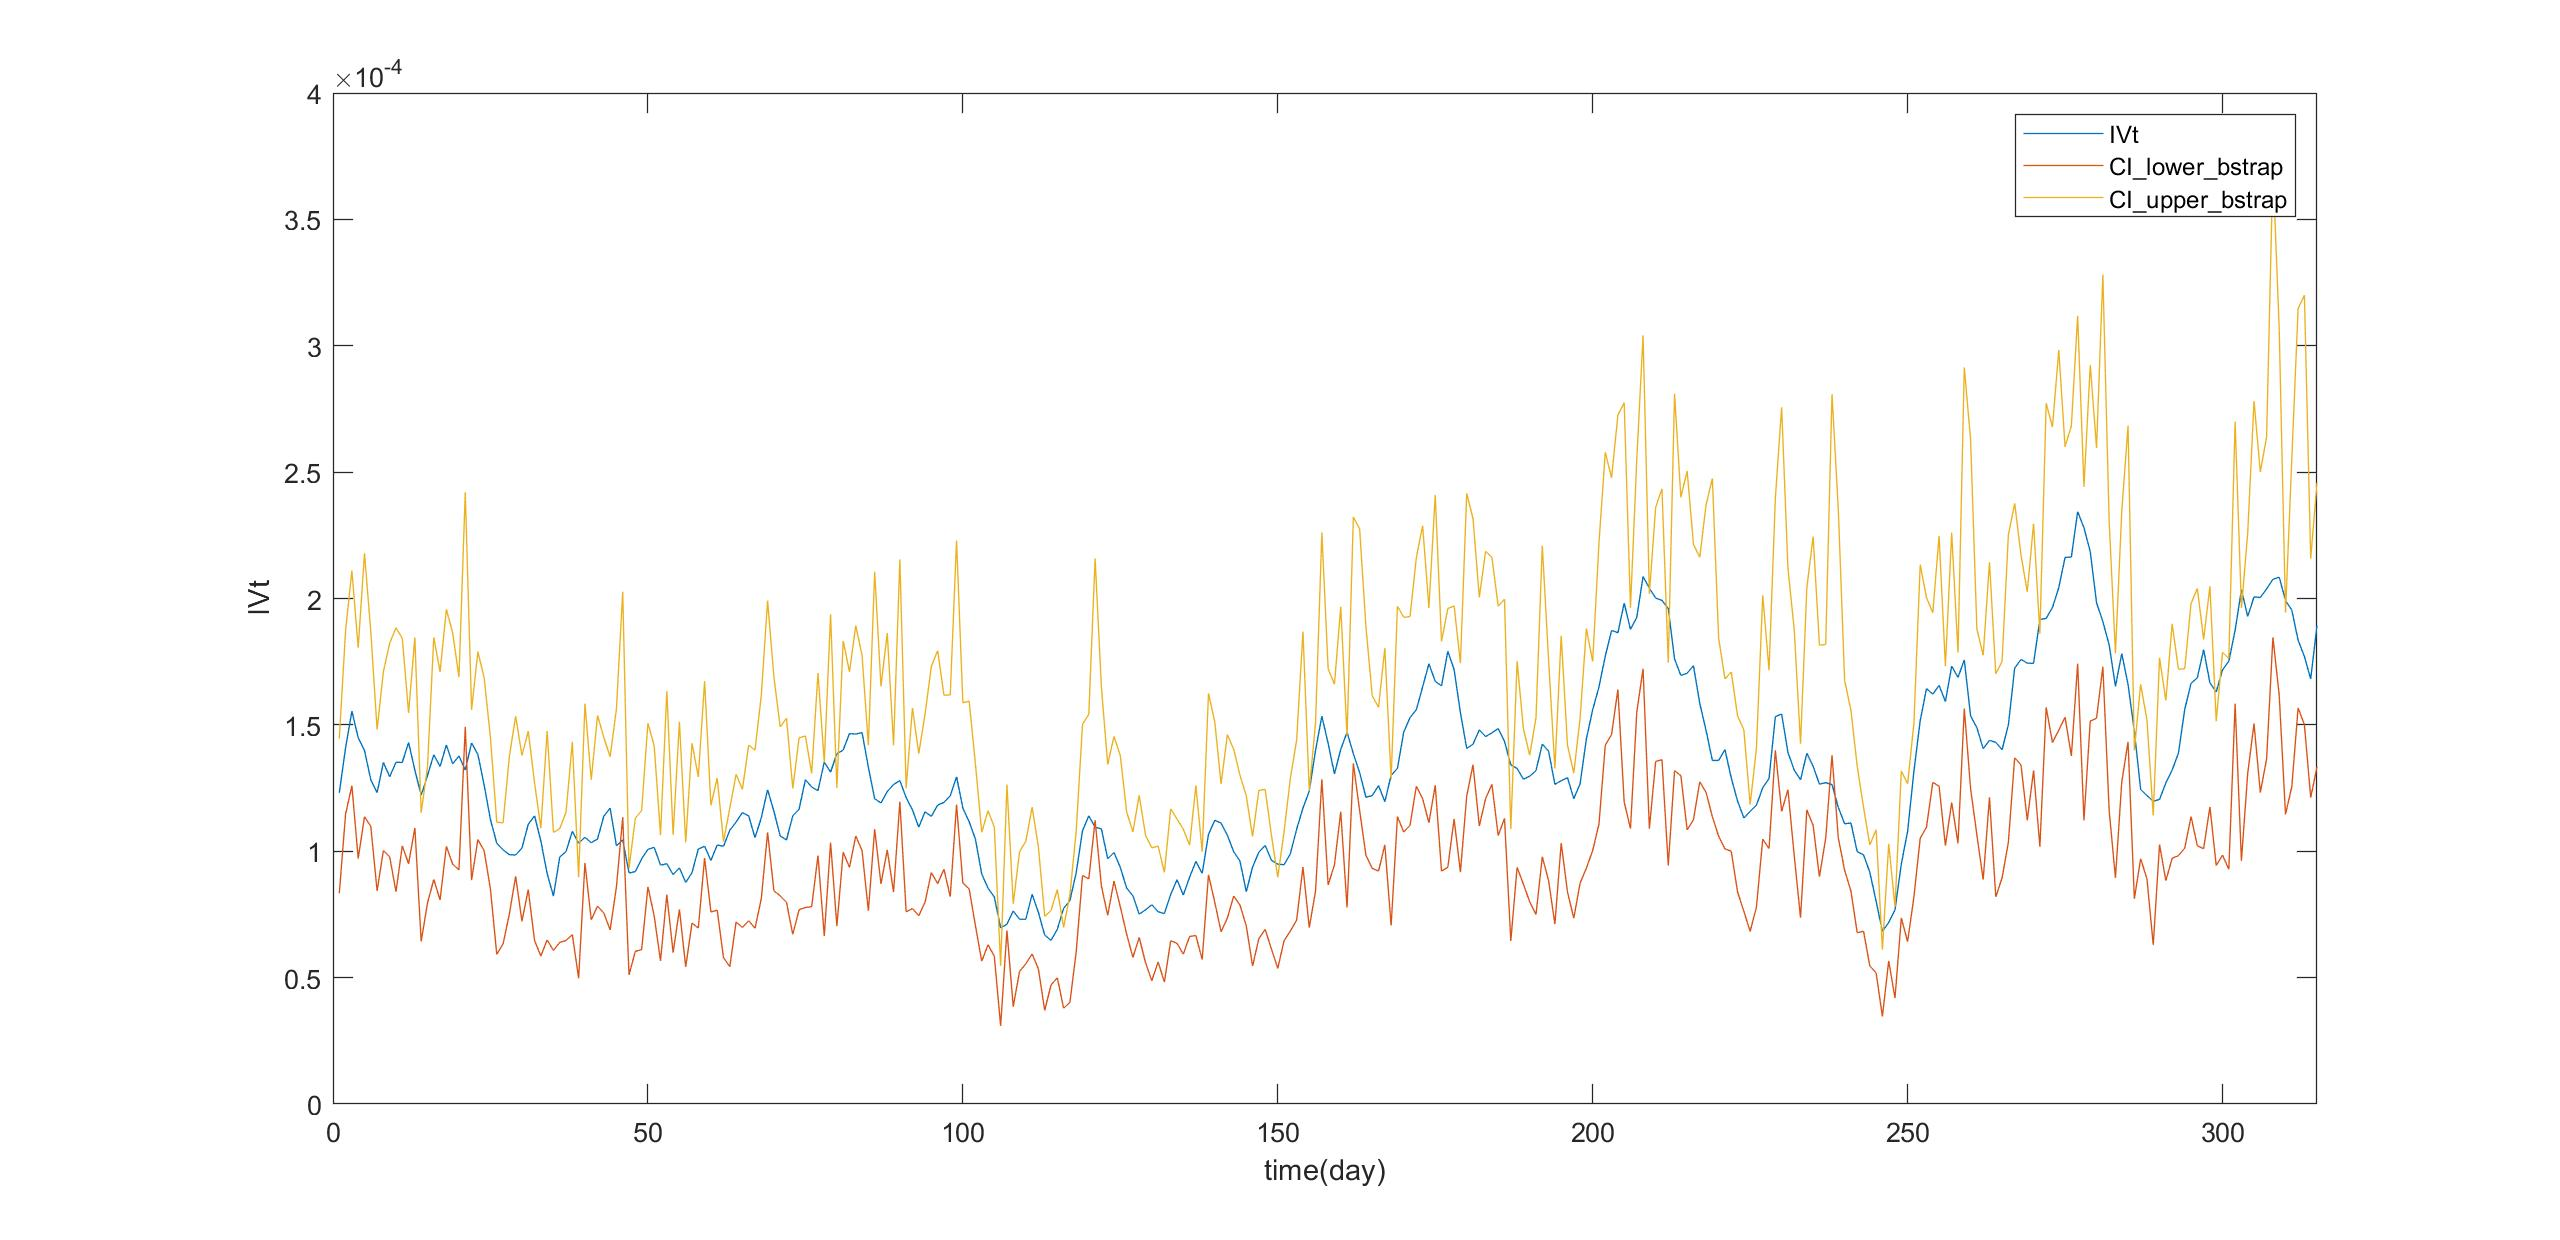
\includegraphics[width=3in]{figures/p4_ex1_f_bs.jpg}
            \end{minipage}
            }
            \centering
            \caption{IV and confidence interval}
\end{figure}

 \begin{figure}[H]
            \centering
            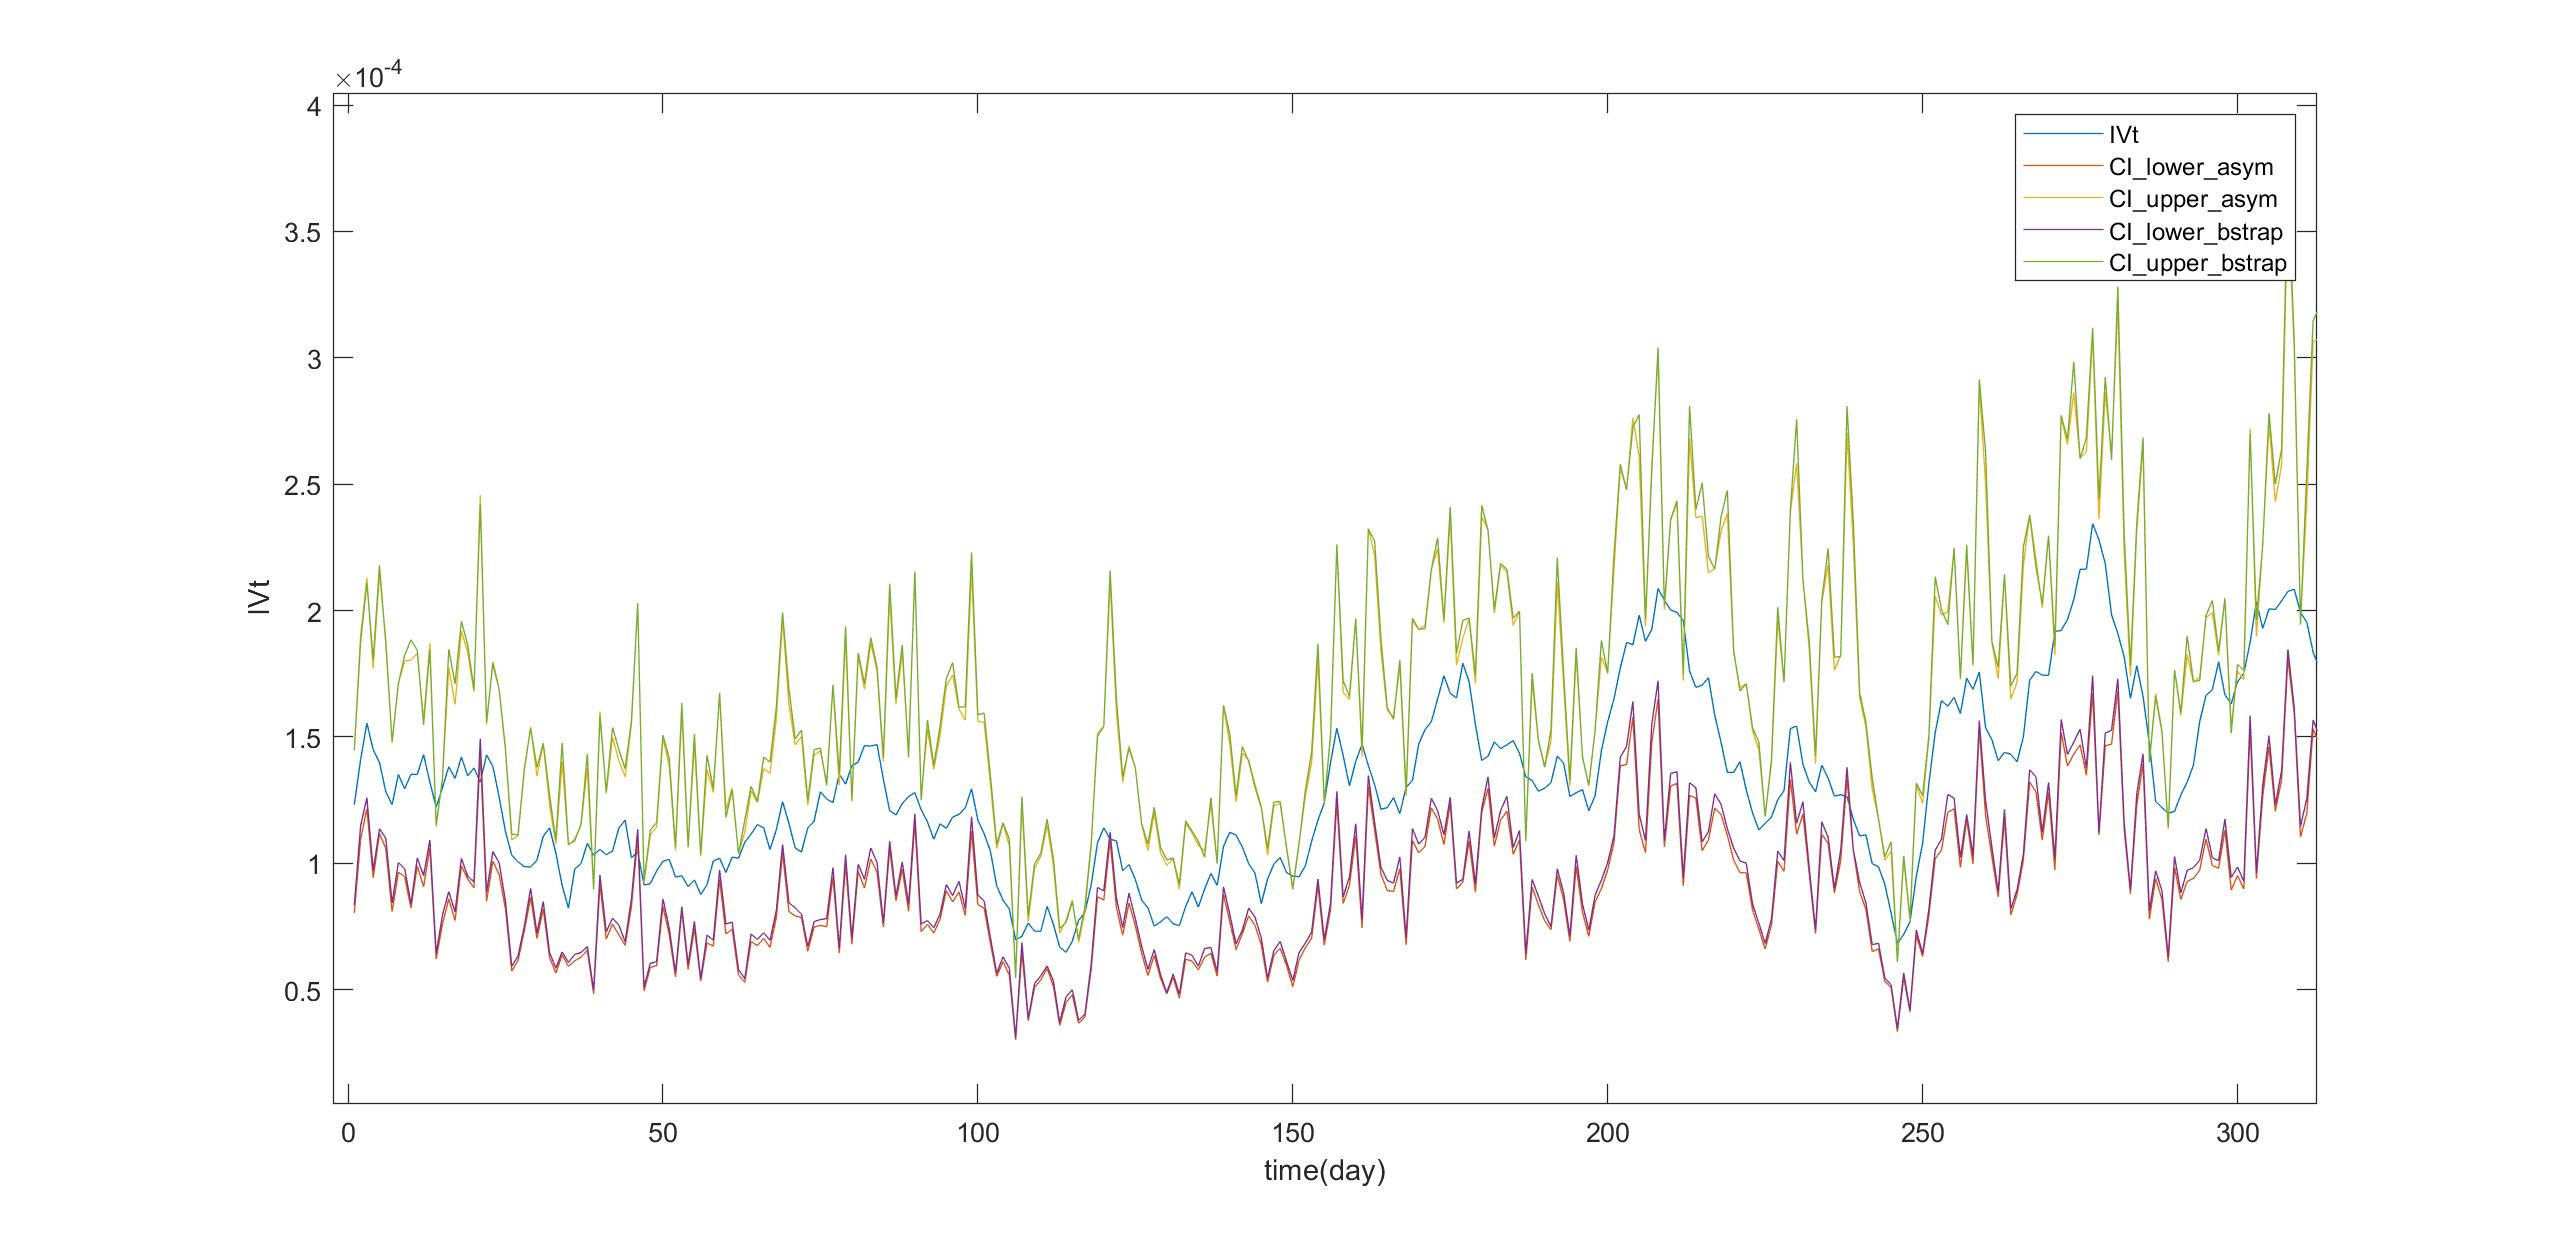
\includegraphics[width=12cm]{figures/p4_ex1_f_3.jpg}
            \caption{IV and CI estimated by asymptotic distribution and bootstrap}
\end{figure}

From these figures we can see, the shape of confidence interval estimated by asymptotic distribution and bootstrap method are very similar, and the value of lower confidence interval and upper confidence interval of bootstrap method are bigger the what we get from asymptotic distribution method. 

The cover number and cover rate for these two methods in one experiment is:
$$Cover\_num_{asym}=291   ~~~~ Cover\_ratio_{asym}=92.38\% $$
$$Cover\_num_{bstrap}=292  ~~~~ Cover\_ratio_{bstrap}=92.70\%$$

The accuracy of distribution asymptotic and bootstrap method to estimate the confidence interval for IV in this case is similar.\\


The \textbf{MATLAB}:
   \lstinputlisting{scripts/p4_ex1_PG.m}
\lstinputlisting{scripts/p4_ex1_f.m}


\end{enumerate}
 

\newpage

%---------------------------------------------

\section*{Exercise 2}
  \begin{enumerate}[label=\textbf{(\Alph*)}]
%---A---
\item The follows are the plot of realized beta of PG and DIS.
\begin{figure}[H]
           \subfigure{
           \begin{minipage}[l]{1\linewidth}
           \centering
            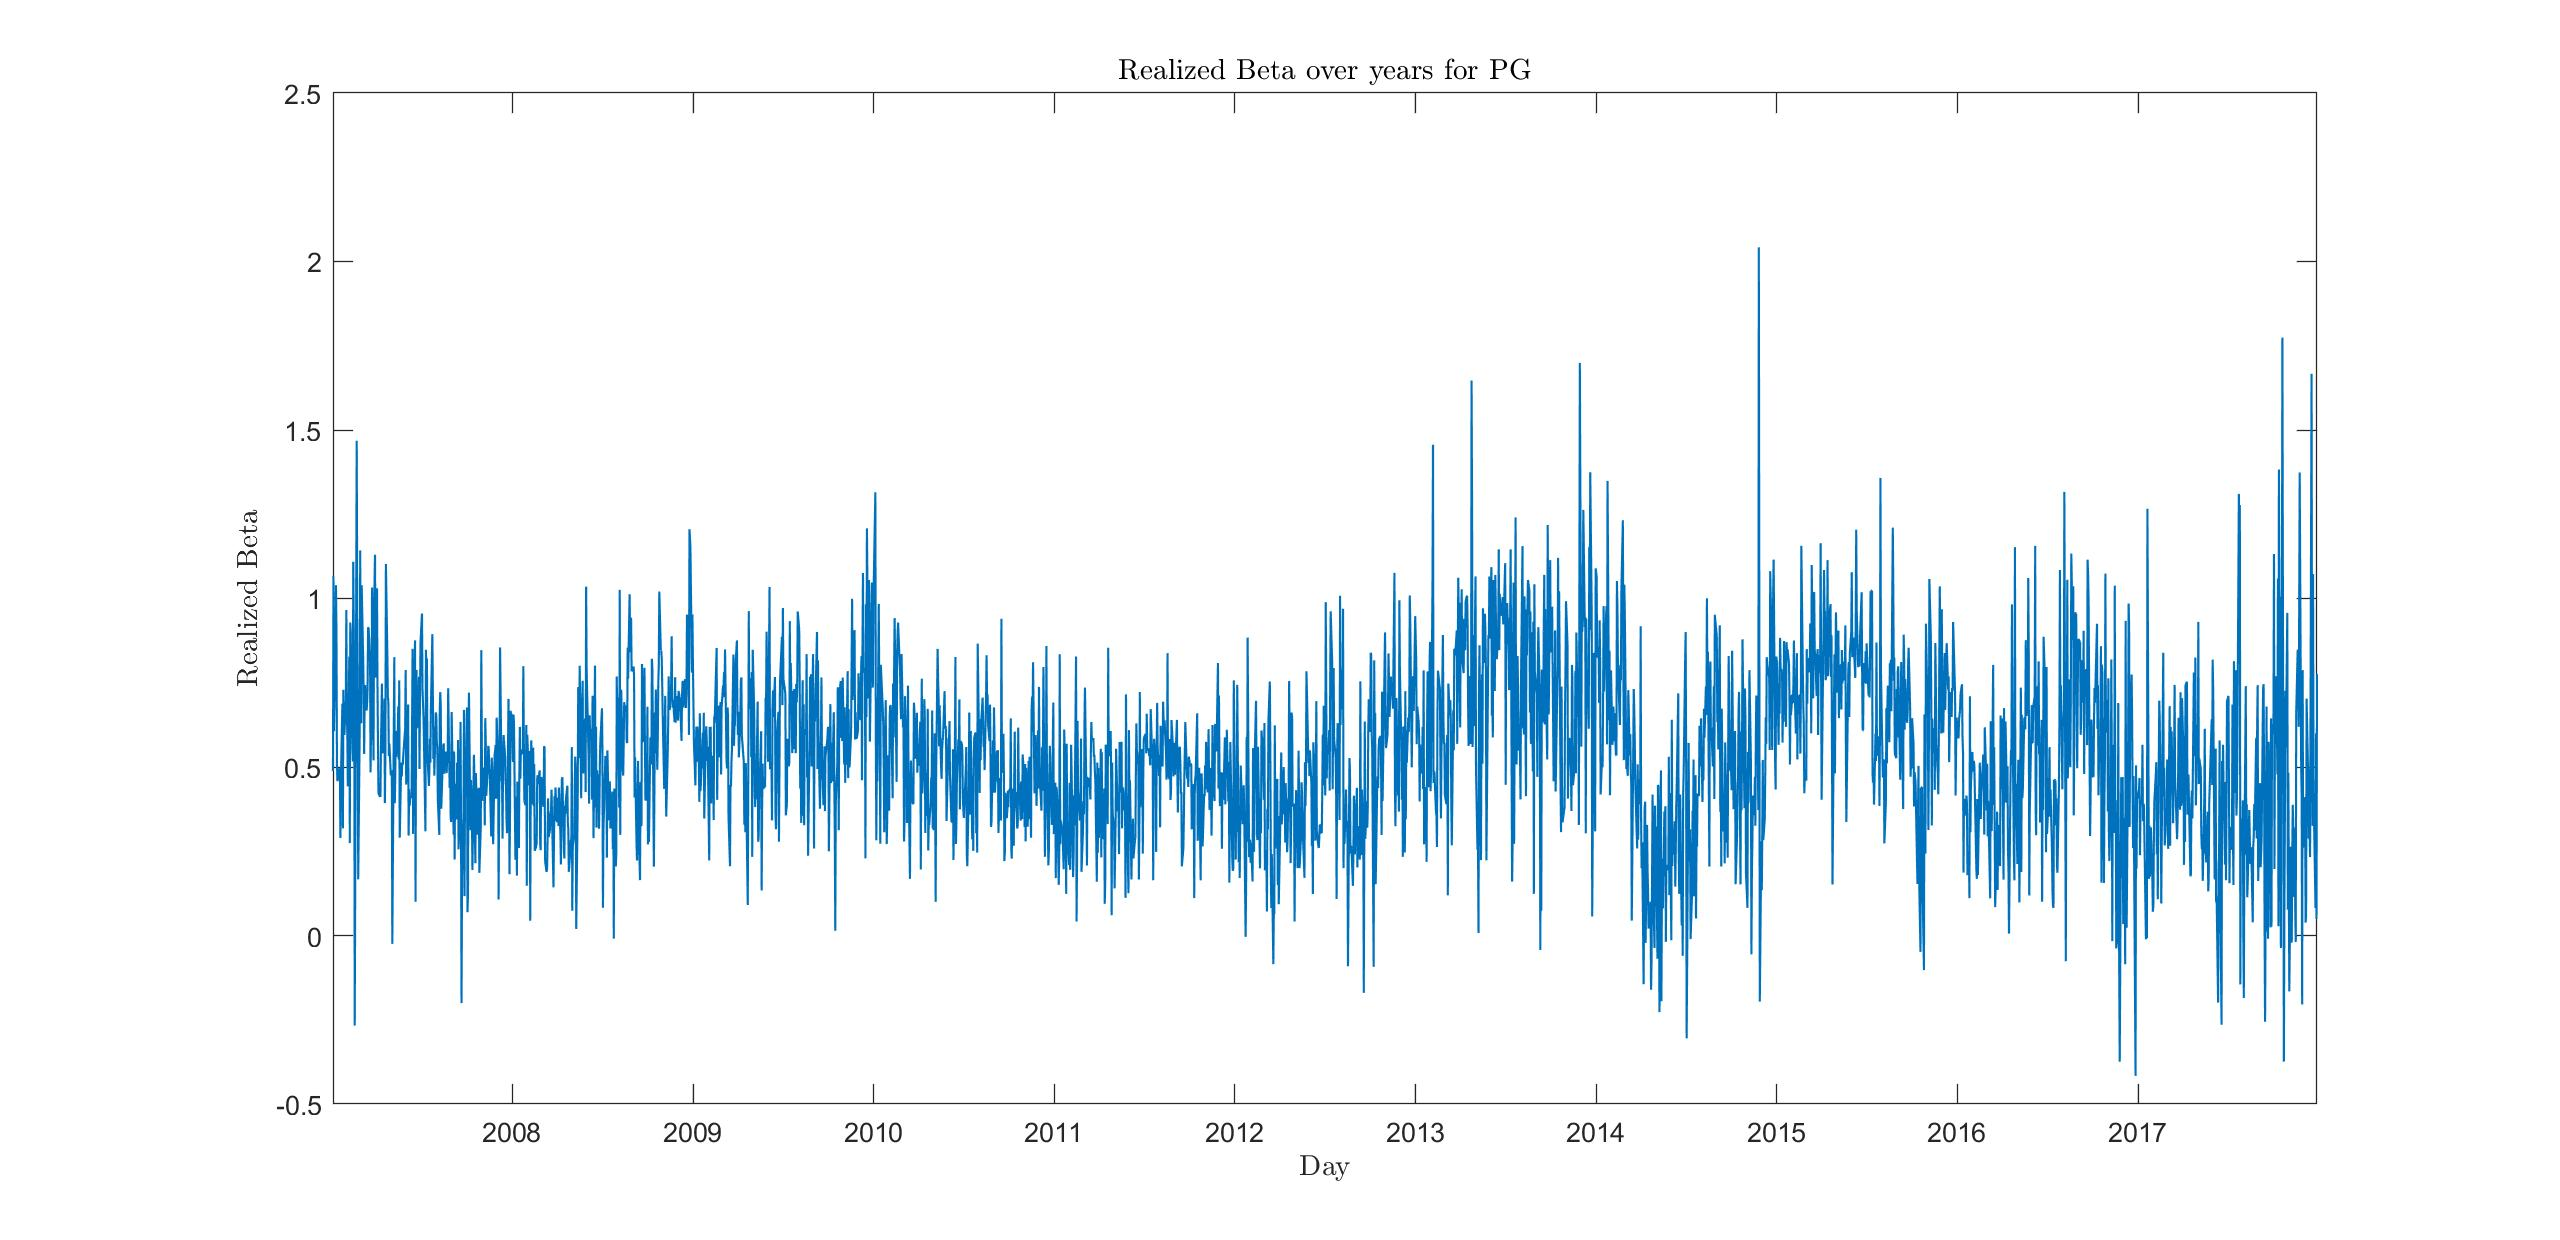
\includegraphics[width=3in]{figures/p4_ex2_a_PG.jpg}
            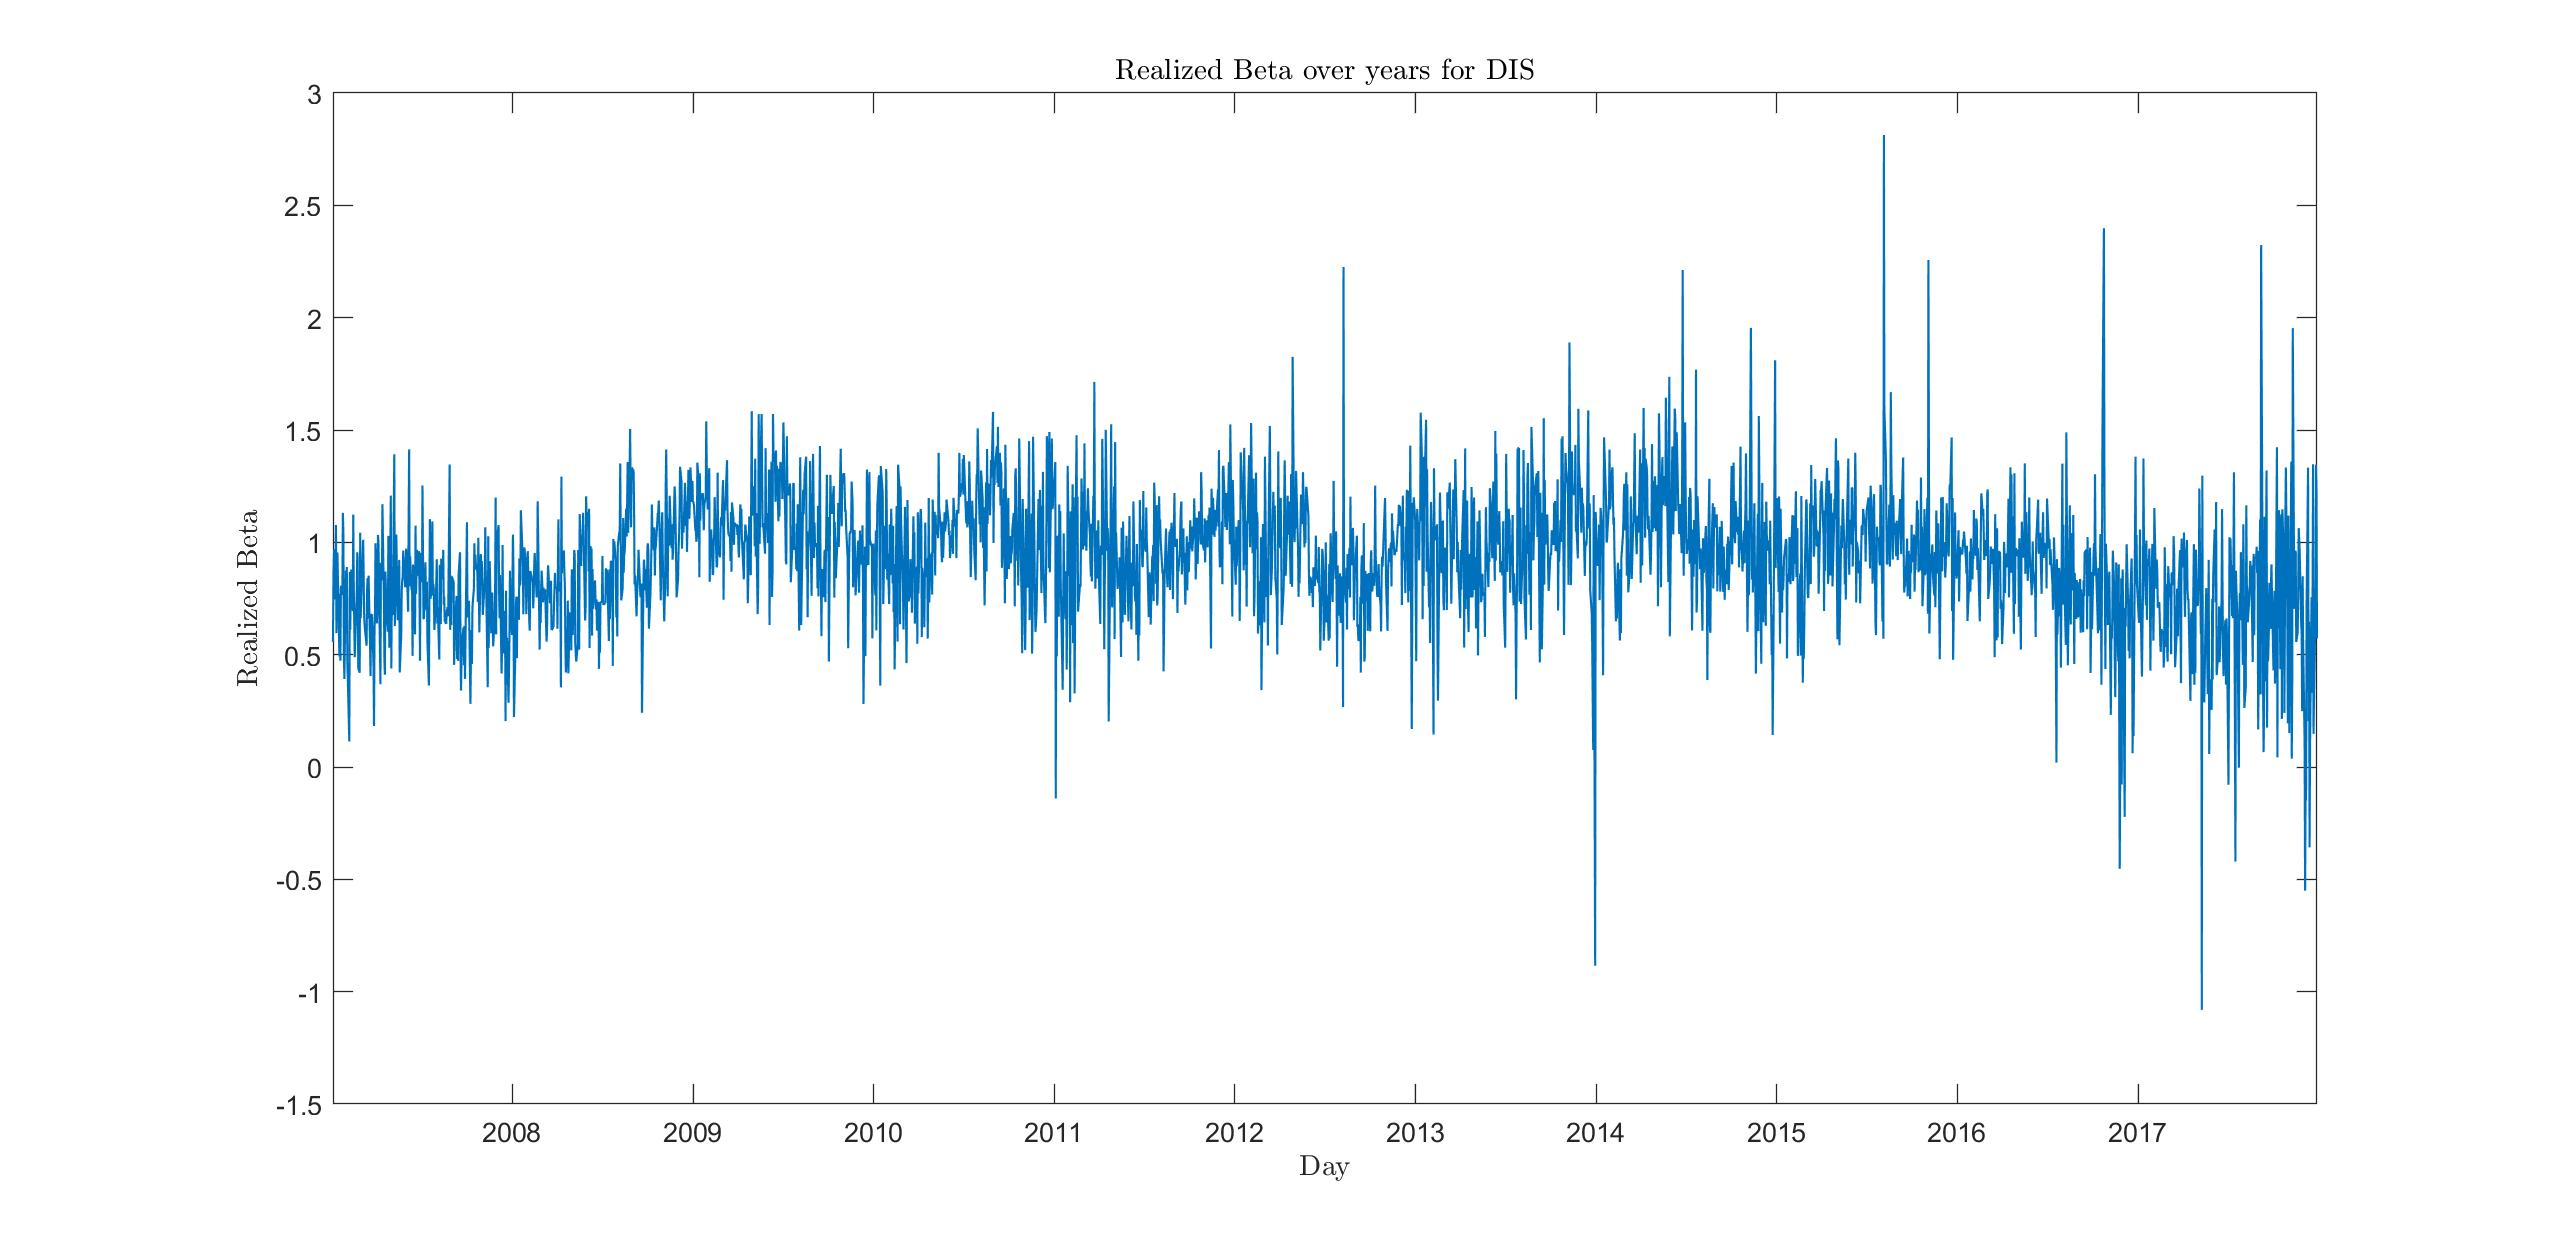
\includegraphics[width=3in]{figures/p4_ex2_a_DIS.jpg}
            \end{minipage}
            }
            \centering
            \caption{Realized beta of PG and DIS}
\end{figure}

From the figure, the realized beta of PG and DIS are volatility and do not show a reasonable stable trend. PG's realized beta mostly falls below the line $R\beta=1$, which means that PG may have a lower beta than the market for most in trading day. This is verse in the case of DIS. As we can see from the figure, most of DIS' realized beta falls above or around the line $R\beta=1$, this indicates that the beta of DIS may have a higher value than market in most of trading day.\\

%----b-----
\item From figures in part A, the value of realized value for both stock vary throughout years. DIS stock's realized beta's volatility is smaller than PG's and we can find a value that the value of DIS' realized bate may move around. However, this isn't enough for us to assume the beta value is fixed. For PG, whose realized beta varies more, this assumption will be even more unreasonable.\\

%-----c-----
\item The follows are the plots of estimated confidence interval of PG and DIS.

\begin{figure}[H]
           \subfigure{
           \begin{minipage}[l]{1\linewidth}
           \centering
            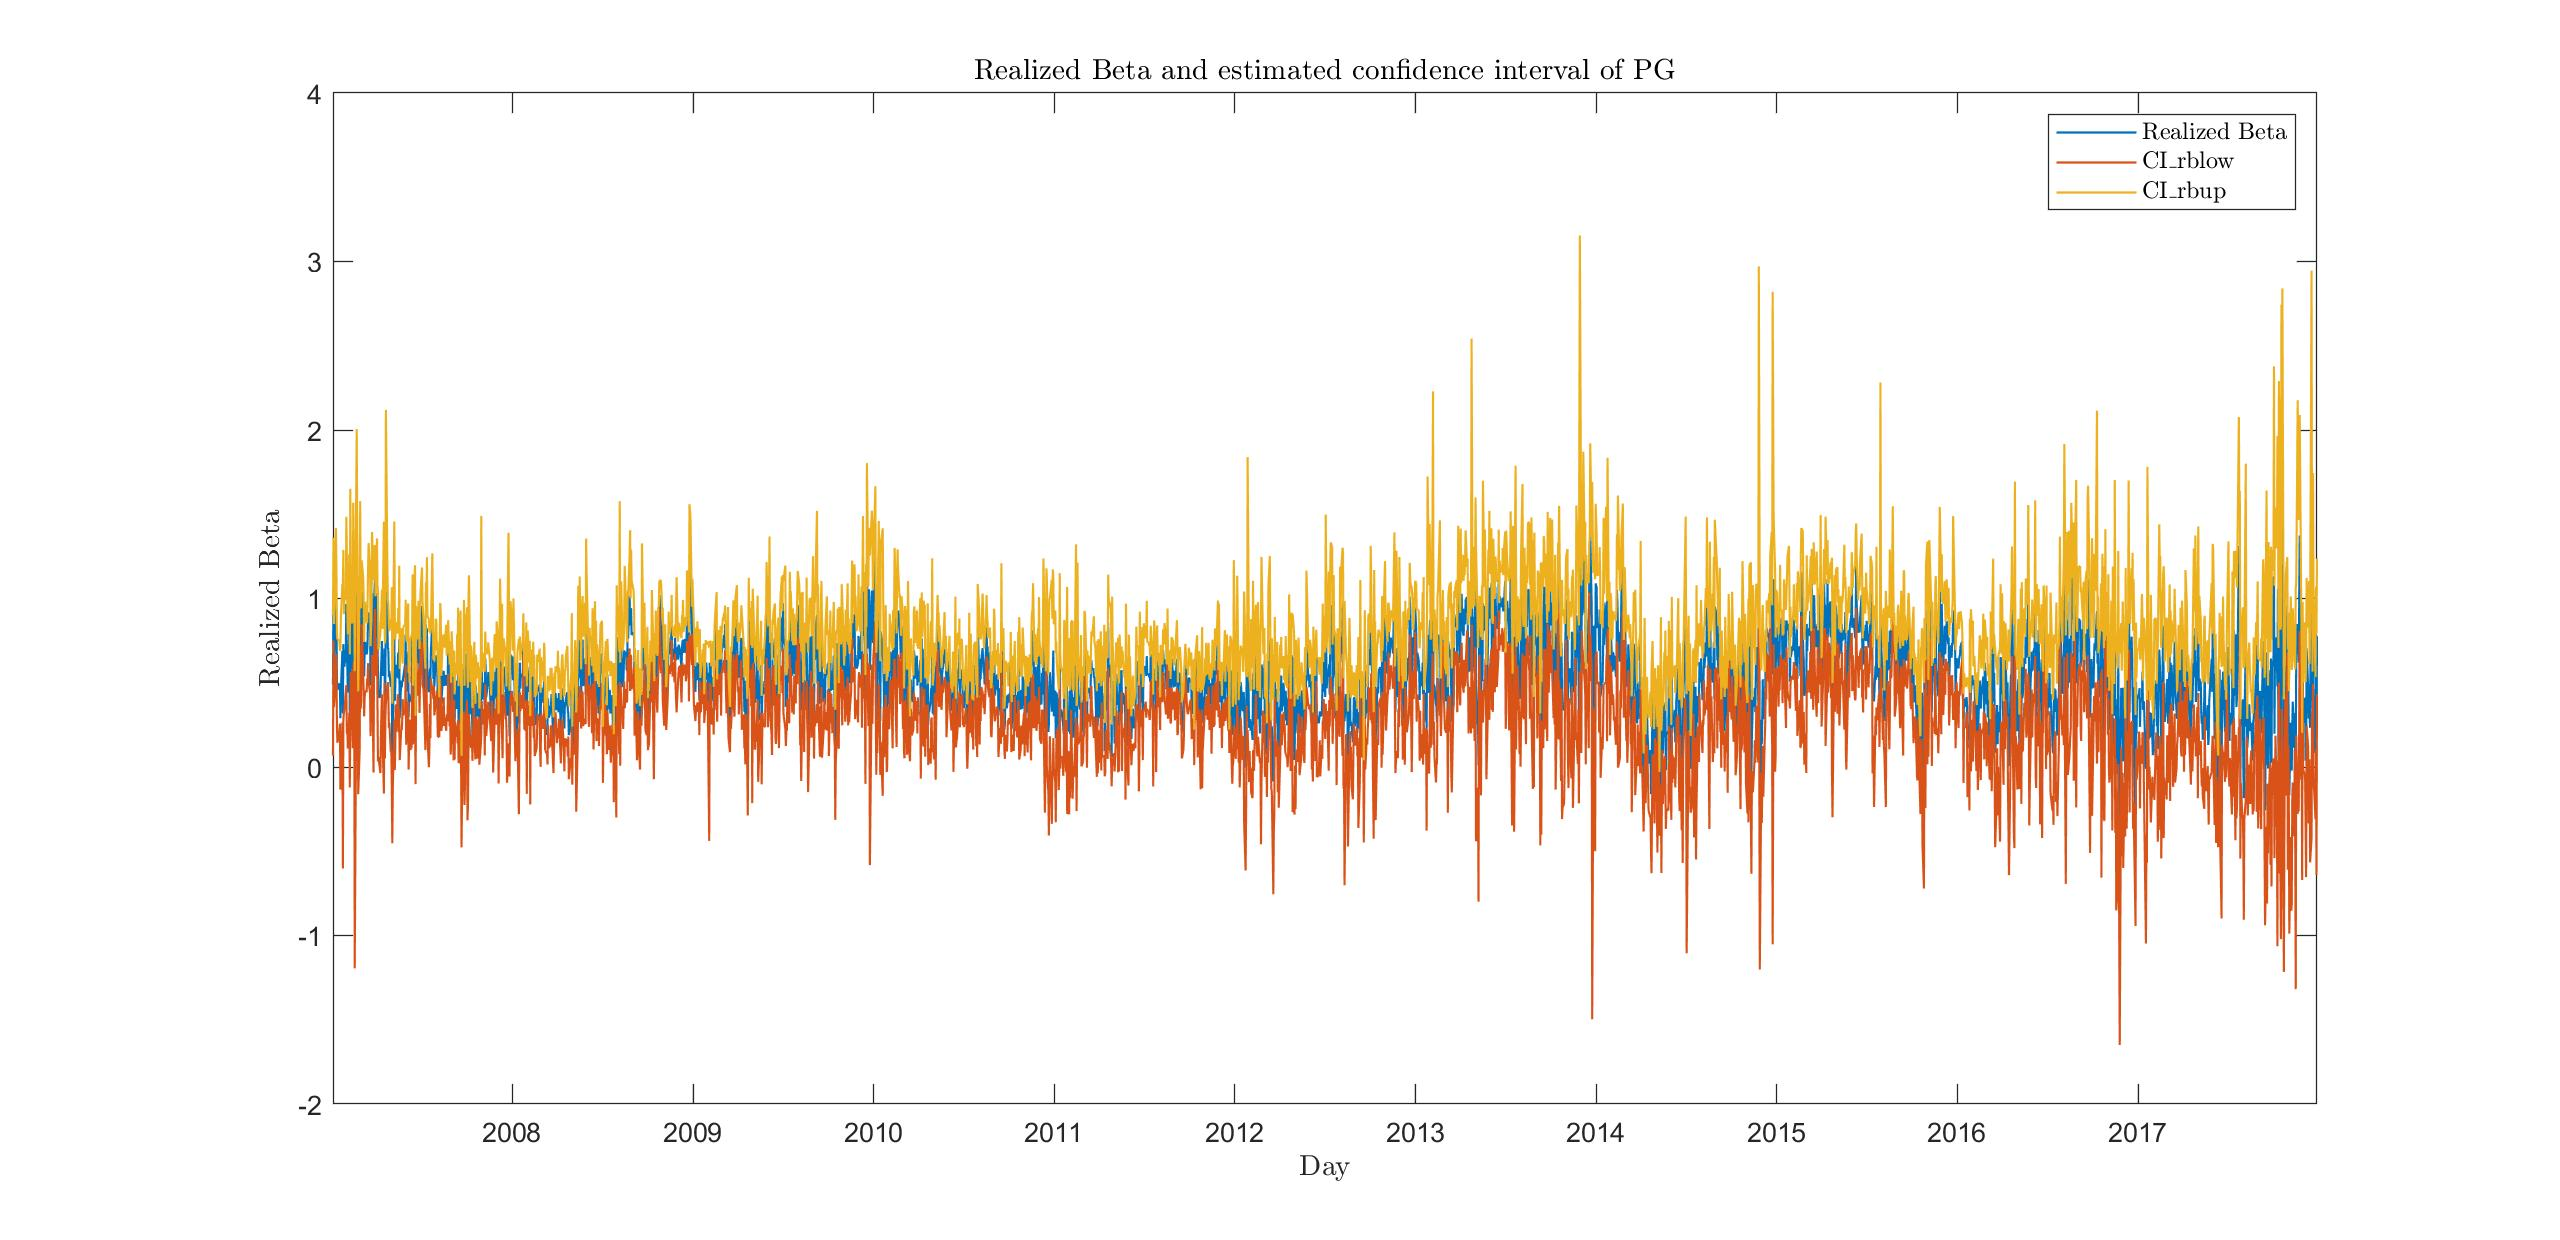
\includegraphics[width=3in]{figures/p4_ex2_c_PG.jpg}
            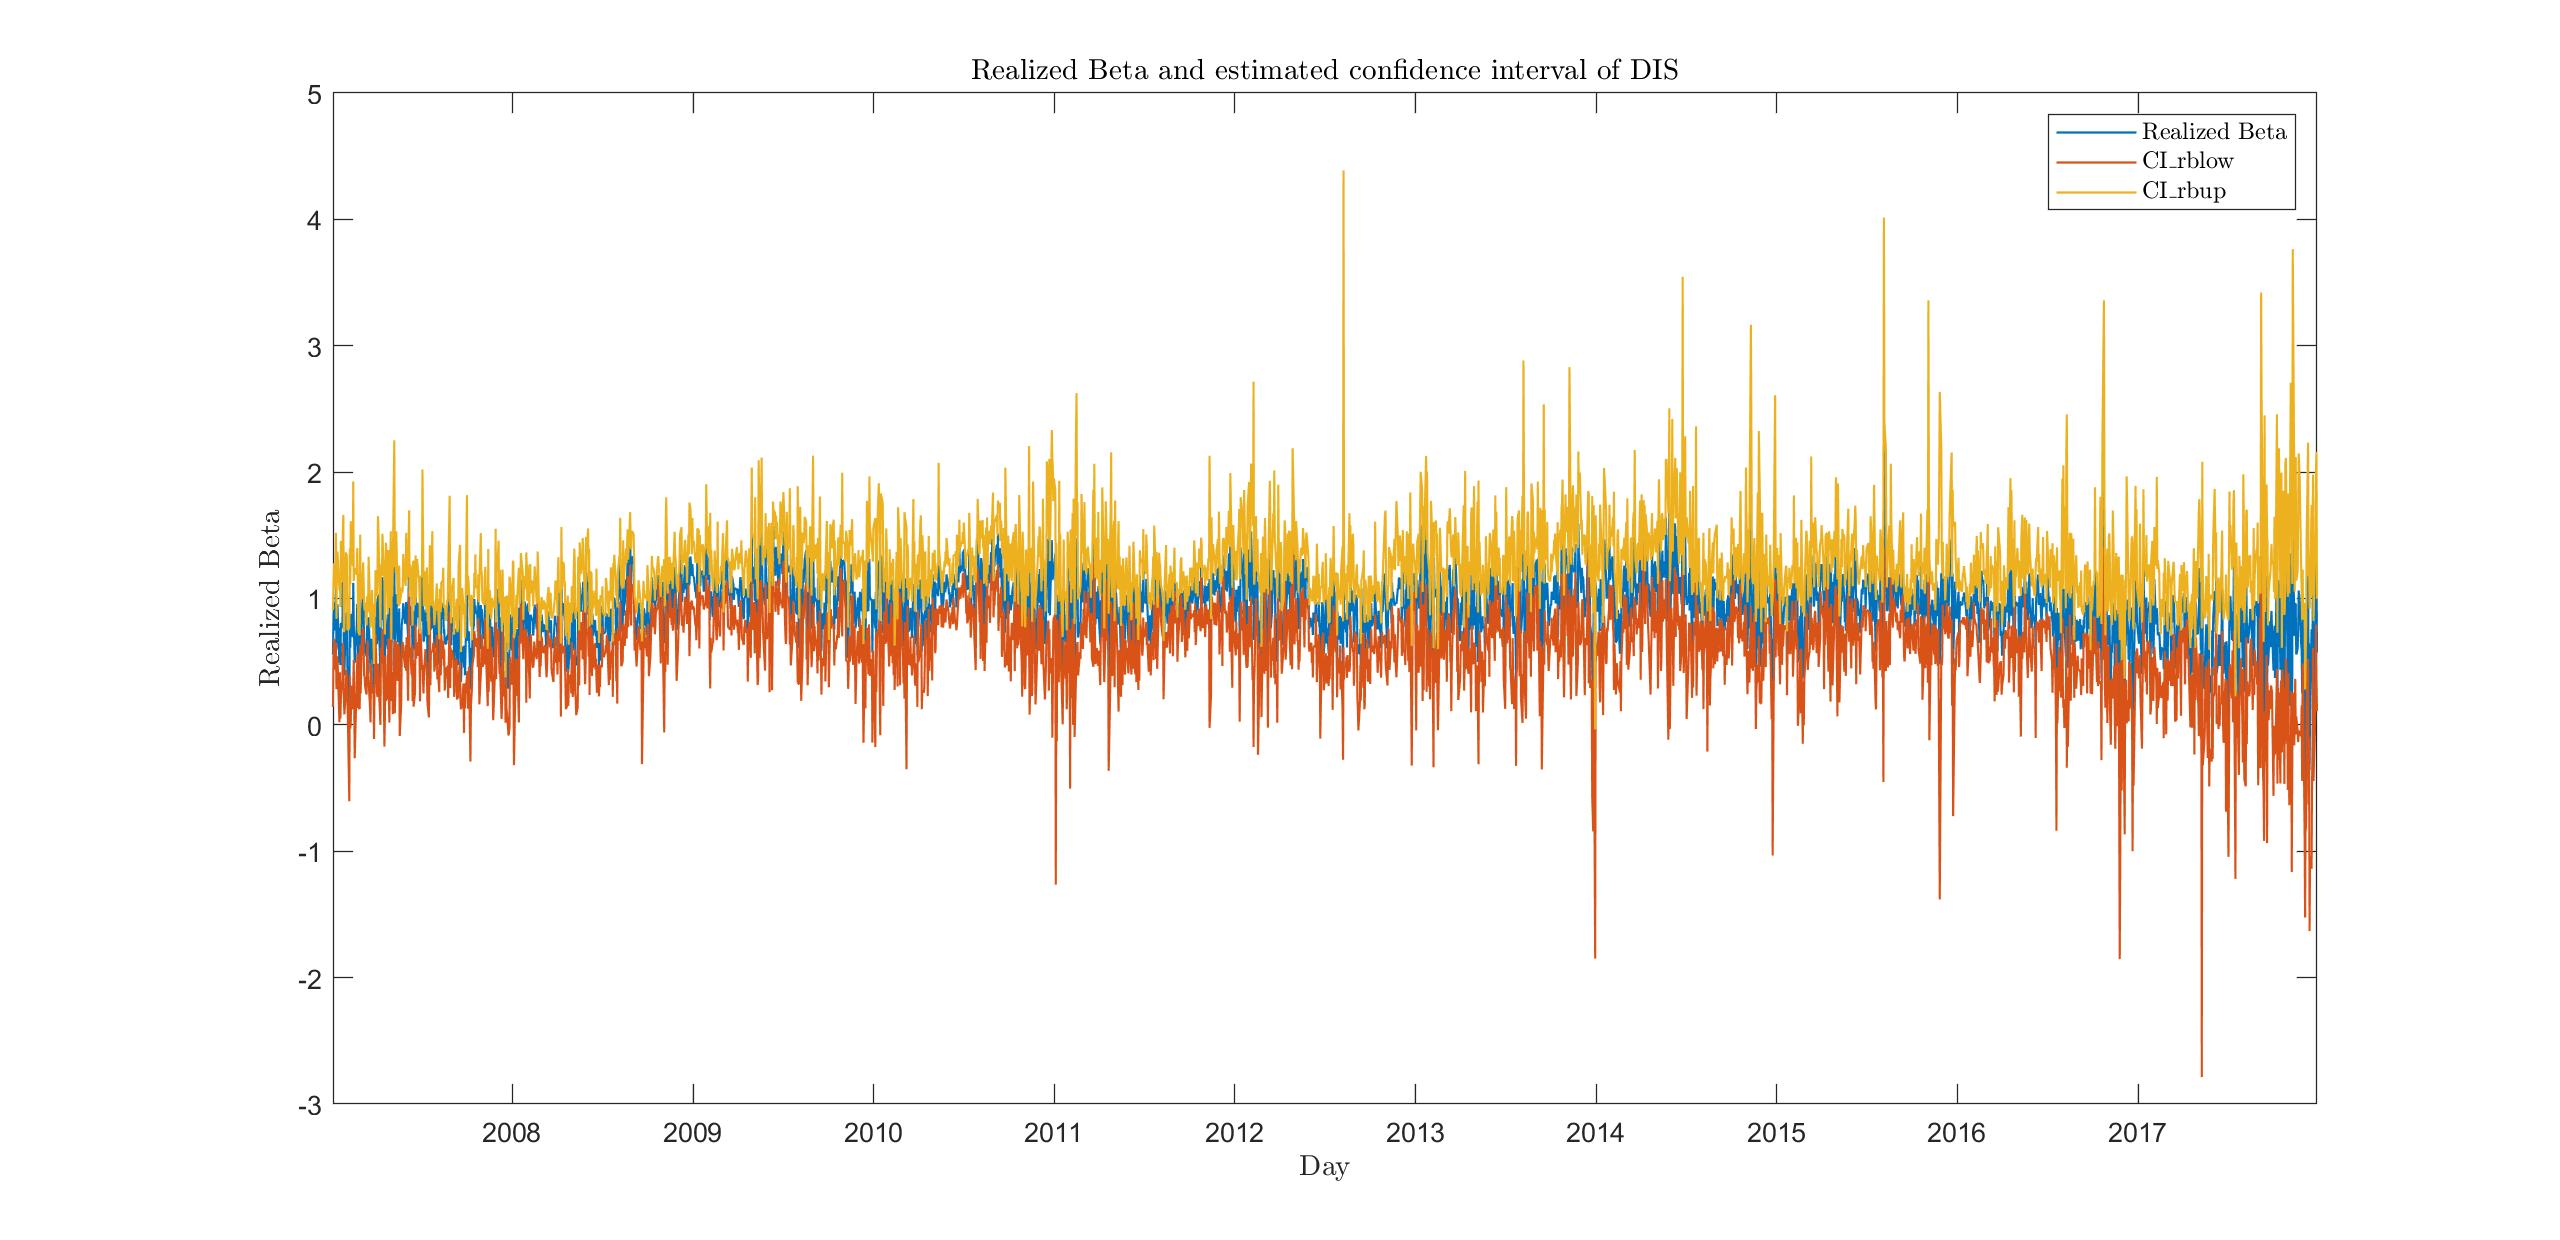
\includegraphics[width=3in]{figures/p4_ex2_c_DIS.jpg}
            \end{minipage}
            }
            \centering
            \caption{Realized beta and estimated confidence interval of realized beta of PG and DIS}
\end{figure}


The number of realized beta of PG falls into estimated confidence interval is 2759 and the cover rate is 99.64\%.The number of realized beta of DIS falls into estimated confidence interval is 2769 and the cover rate is 100\%. This result indicates that the estimated confidence interval is good and the accuracy of using bootstrap to estimate the confidence interval is higher than the method of using asymptotic distribution. \\

%----d----
\item The follows are the figures of realized beta of PG and DIS in January 2007.

\begin{figure}[H]
           \subfigure{
           \begin{minipage}[l]{1\linewidth}
           \centering
            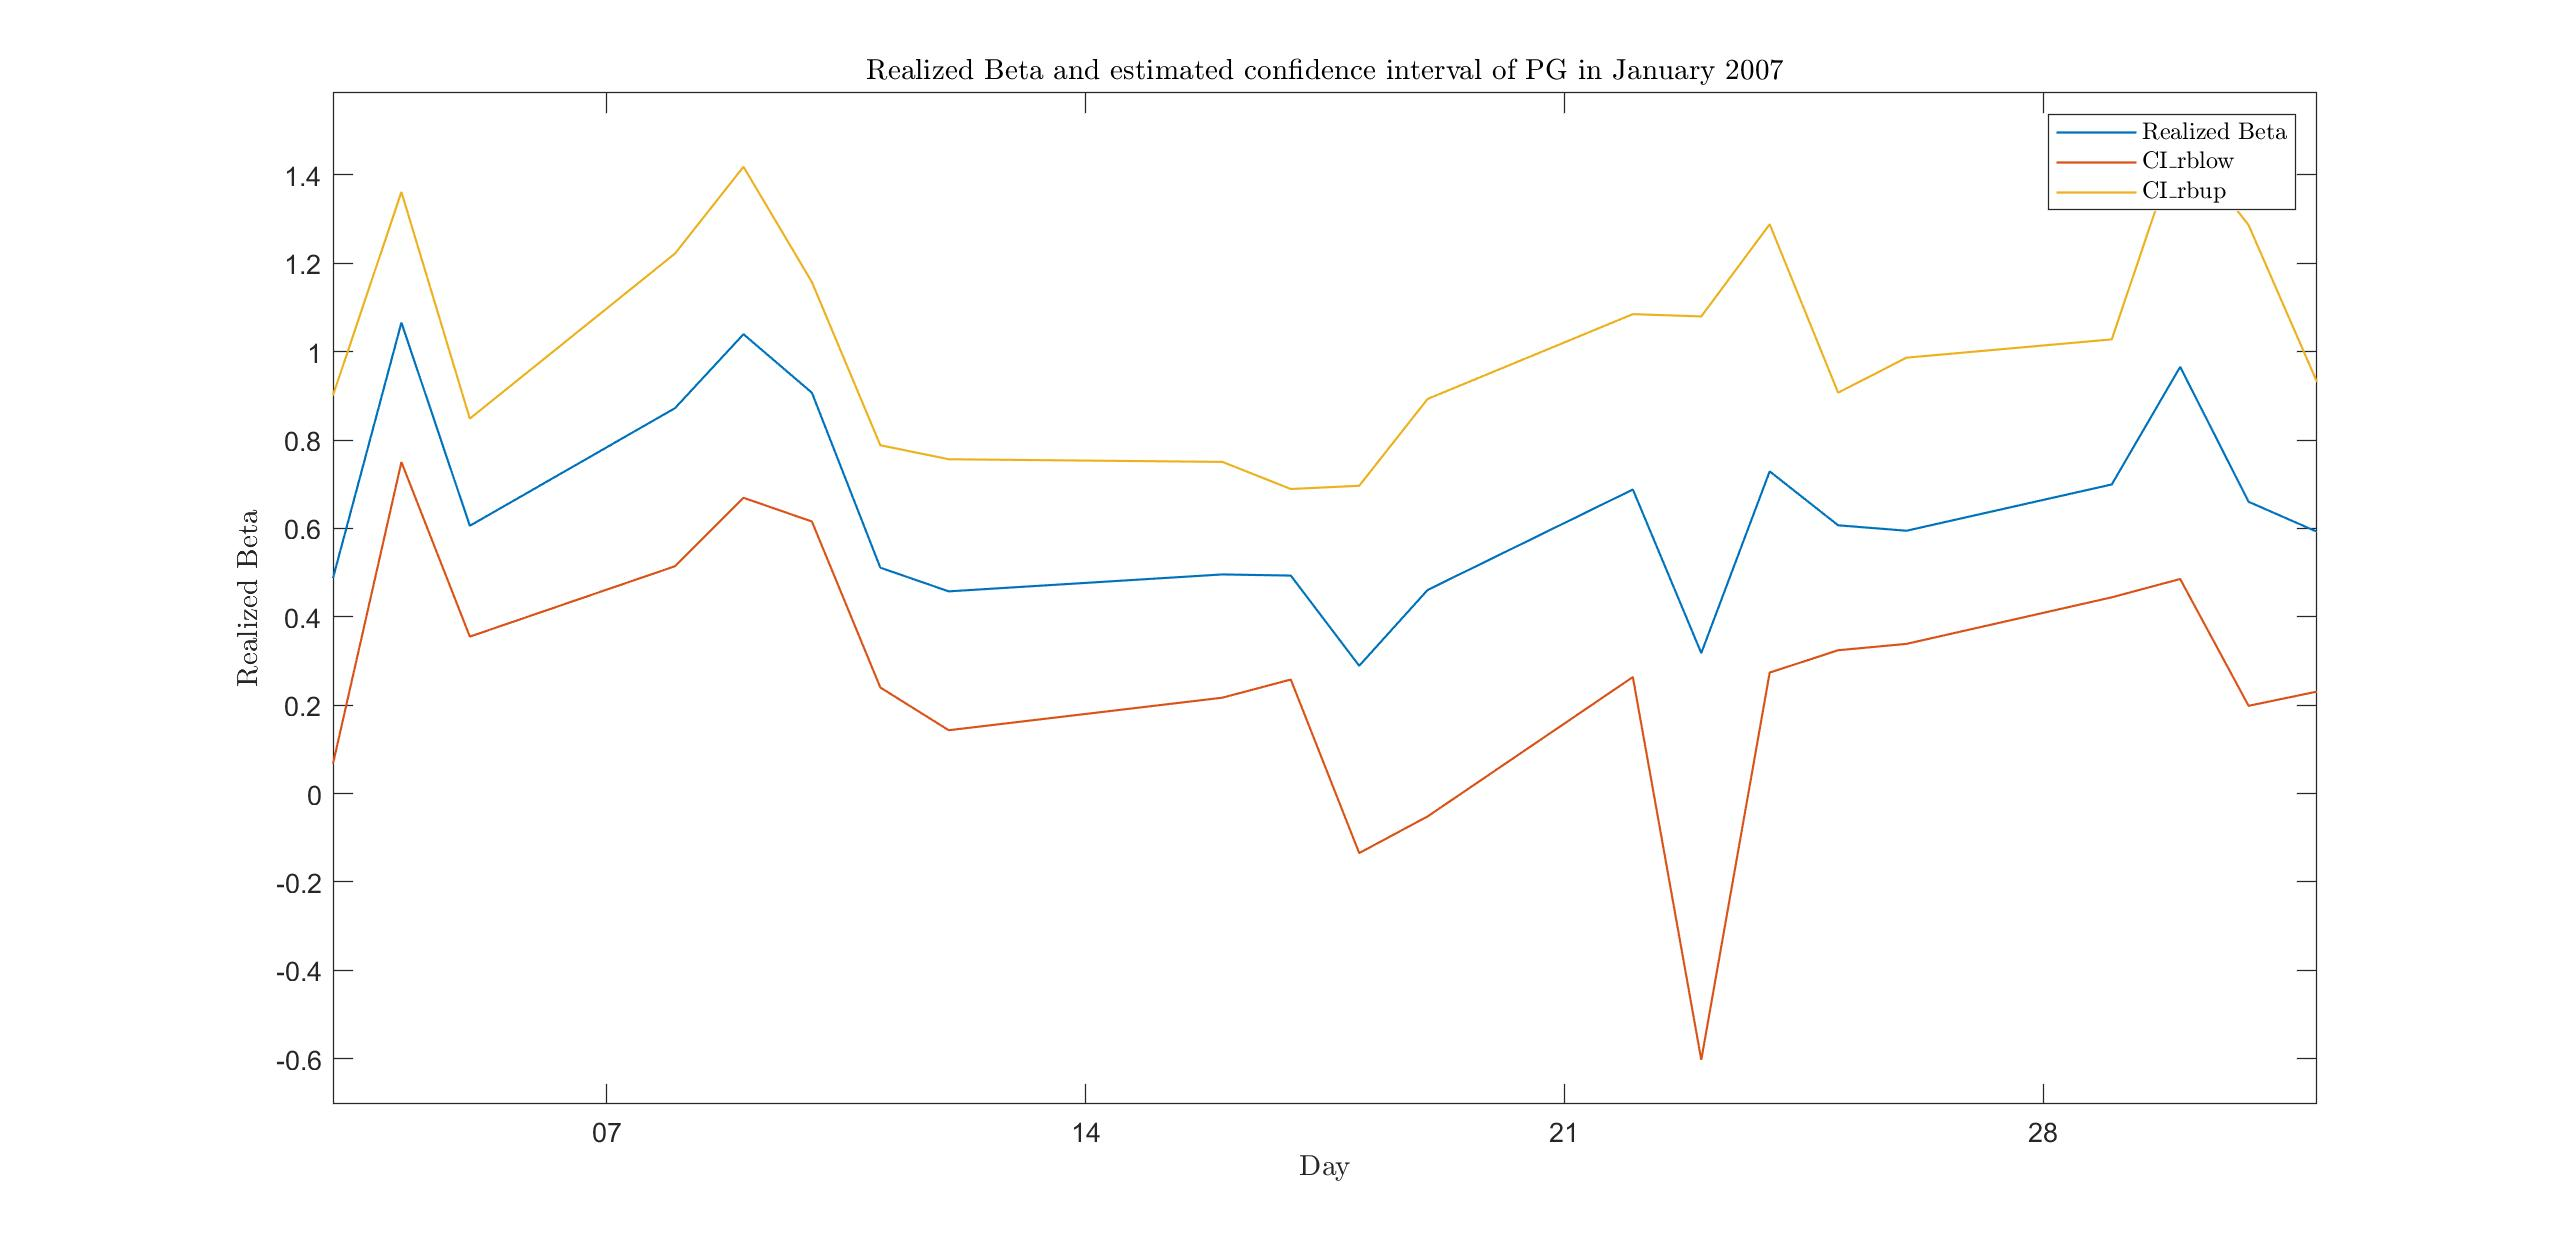
\includegraphics[width=3in]{figures/p4_ex2_d_PG.jpg}
            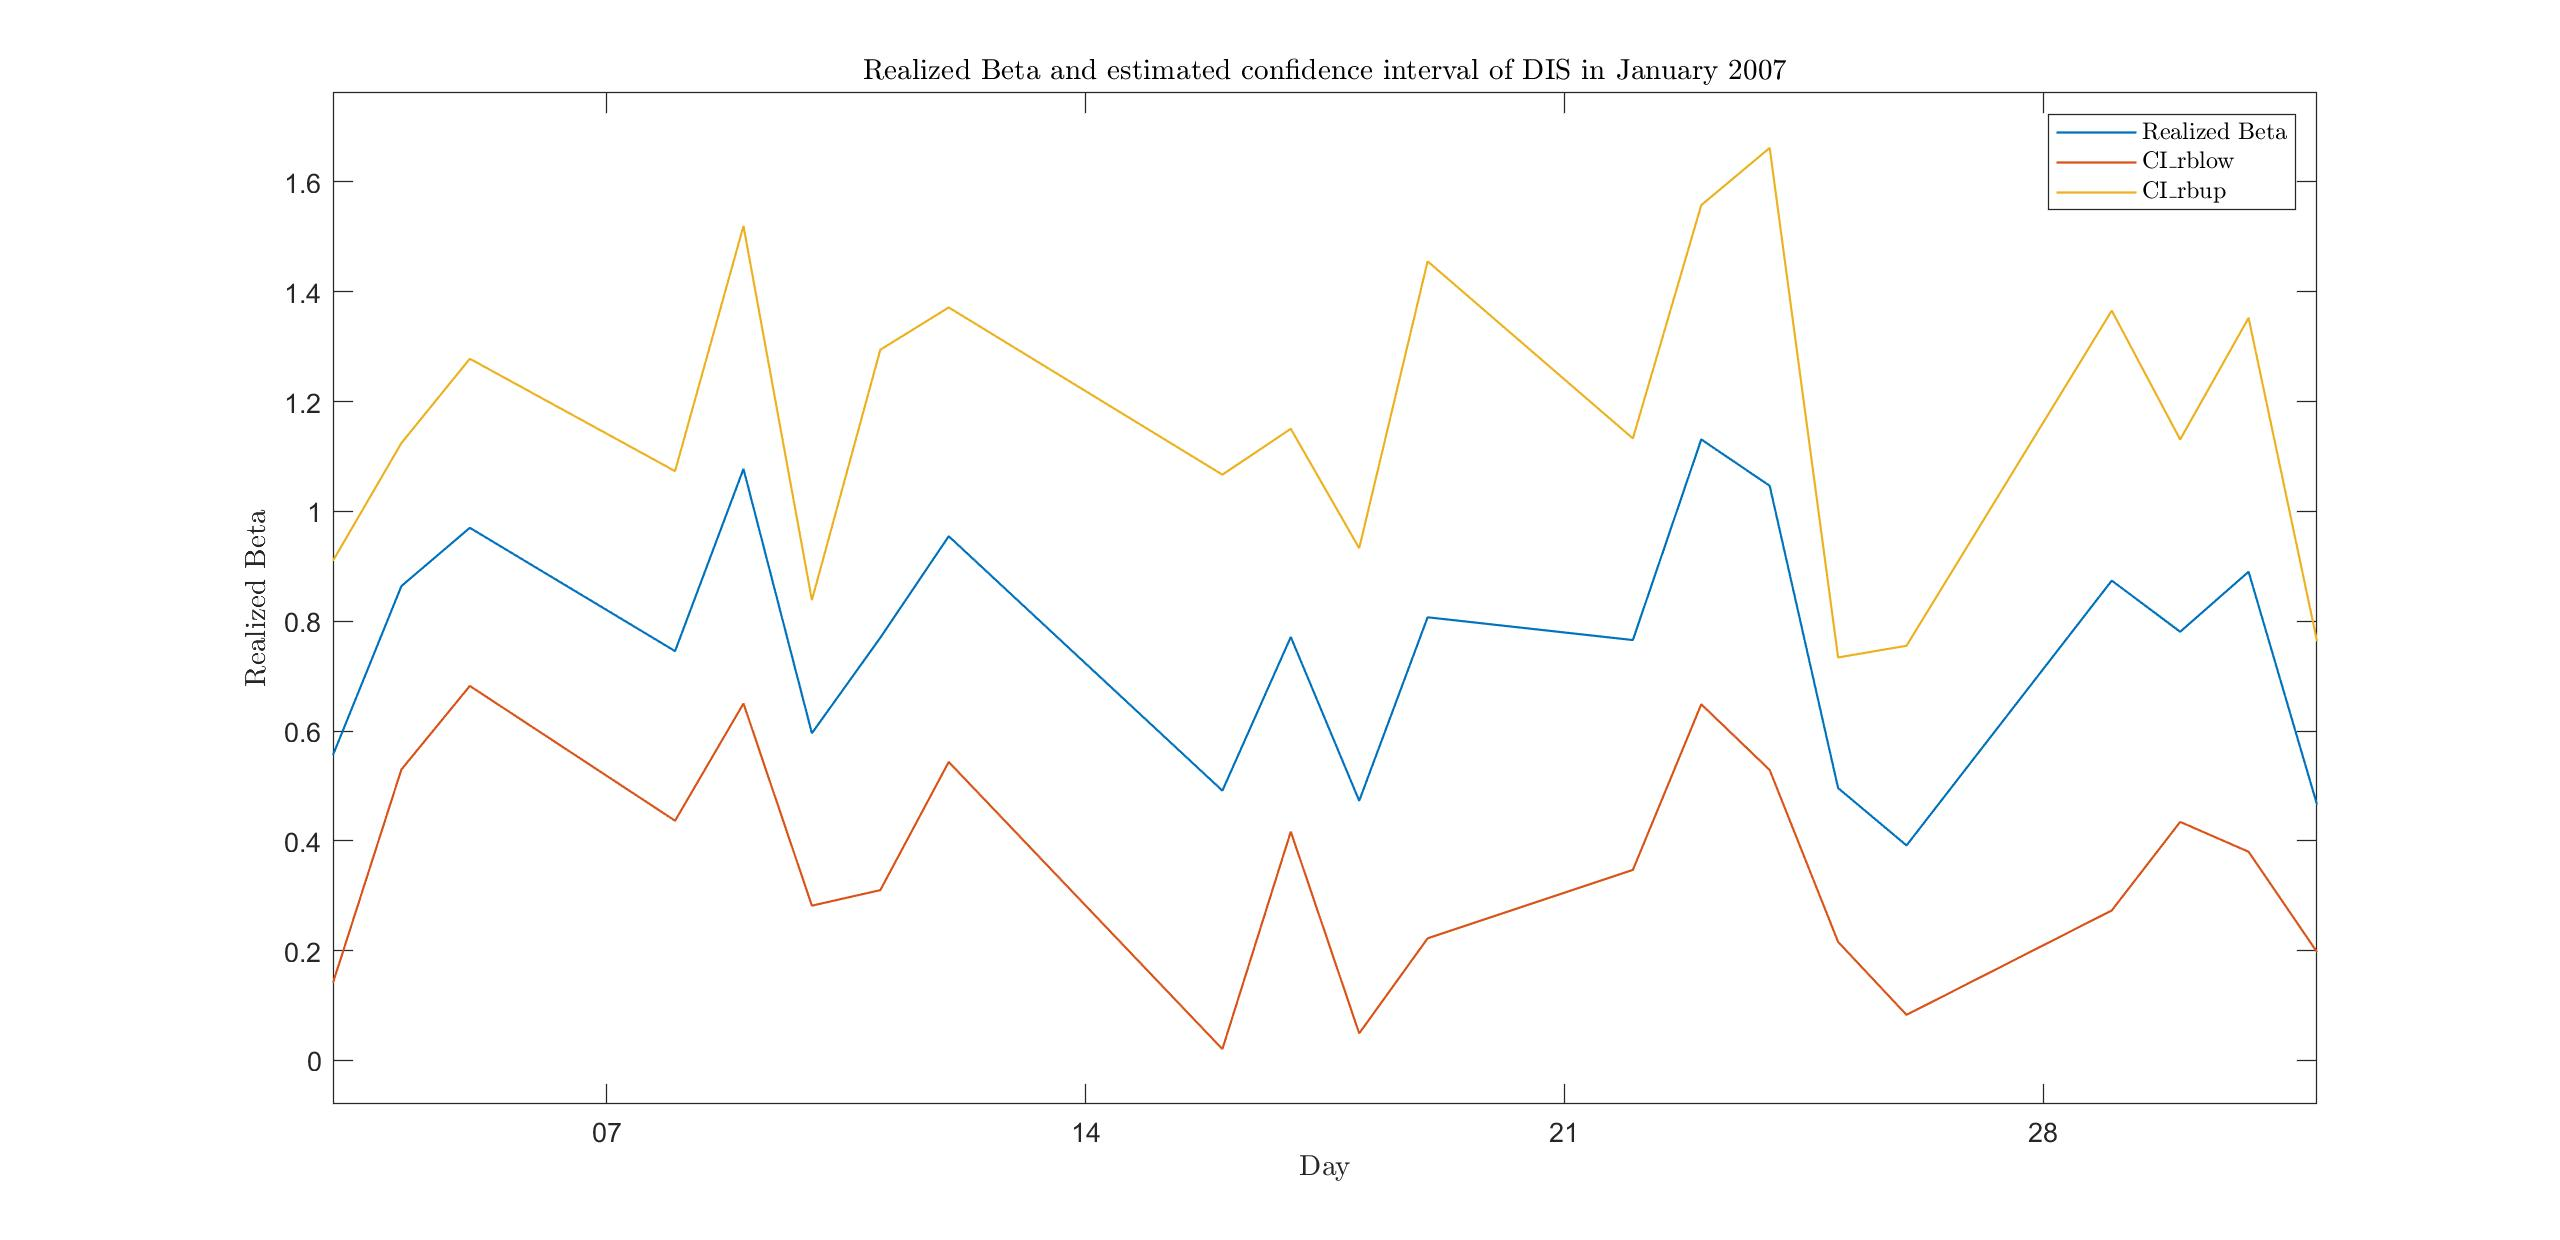
\includegraphics[width=3in]{figures/p4_ex2_d_DIS.jpg}
            \end{minipage}
            }
            \centering
            \caption{R$\beta$ and estimated CI of PG and DIS in January 2007}
\end{figure}

We can see form the figures that, the estimated confidence interval bounds the realized beta for both PG and DIS well. Look closer to the shape of confidence interval, we can find that the shape of upper bound and the lower bound is a little different, while the shape of upper bound and lower bound we get from asymptotic distribution method is similar. \\
  
%----e-----
\item 
\begin{enumerate}[label=(\roman*)]
    \item The confidence interval contains 1: $N_{1\_PG}=648$ and $N_{1\_DIS}=2091$.
    \item The confidence interval is below 1: $N_{<1\_PG}=2118$ and $N_{<1\_DIS}=477$.
    \item The confidence interval is above 1: $N_{>1\_PG}=3$ and $N_{>1\_DIS}=201$.\\
    
\end{enumerate}

For PG stock, the number of confidence interval below 1 takes up 76.49\%, which indicates PG stock will probably have a lower beta than the market for most of its trading day. A lower beta value means that the stock is less volatility than the market and has a lower risk and returns. 
For DIS stock, the number of confidence interval above or equal to 1 takes up 92.74\%, which indicates DIS stock will probably have a higher or equal beta with the market for most of its trading day. A higher beta value means that the stock is more volatility than the market and has a higher risk and returns. \\

The \textbf{MATLAB}:
   \lstinputlisting{scripts/p4_ex2_PG.m}
\end{enumerate}
\newpage


\end{document}
